\chapter{Simulation Results}


This chapter contains the results of some selected examples.
First we show that the code works correctly by simulating
the well known toy examples like harmonic oscillators in different
settings. Next we reproduce some less trivial results from \cite{FGL_semiclassical_dynamics}
in two space dimensions. Finally we show several results of non-adiabatic
transition in two and more space dimensions.

All simulations were performed with our \texttt{WaveBlocksND} simulation
code\cite{waveblocksnd}. The code can perform simulations with an arbitrary
number $N$ of energy levels defined in an arbitrary number $D$ of space
dimensions. The only limitations are available computer memory and time.


\section{Harmonic oscillators}


The harmonic oscillator is the first toy example one usually studies to
check if a new simulation code works as expected. This is also what we
are going to do next. We start with a Gaussian wavepacket having the
parameters:

\begin{align*}
  \vec{q} = \begin{pmatrix}
              1.8 \\ 1.2
            \end{pmatrix}
  \quad
  \vec{p} = \begin{pmatrix}
              0.6 \\ 0.8
            \end{pmatrix}
  \quad
  \mat{Q} = \begin{pmatrix}
              1 & 0 \\ 0 & 1
            \end{pmatrix}
  \quad
  \mat{P} = \begin{pmatrix}
              i & 0 \\ 0 & i
            \end{pmatrix}
  \quad
  S = 0 \,.
\end{align*}

The scaling parameter $\varepsilon$ is set to $0.1$. These values for $\Pi$
result in a cyclic oscillation with elliptical orbits, see figure \ref{fig:ho_traject_q}.
The potential is given by:

\begin{equation}
  V(x,y) \assign \frac{1}{2} \left( \frac{1}{2} x^2 + \frac{1}{2} y^2 \right) \,.
\end{equation}

\begin{figure}
  \centering
  \subfloat[][]{
    \label{fig:ho_energies}
    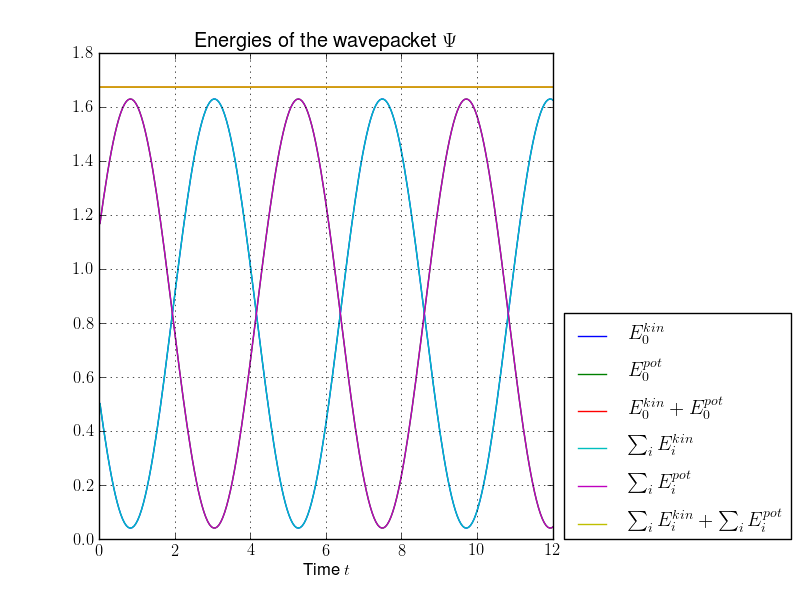
\includegraphics[width=0.5\linewidth]{./results/HO/energies_block0.png}
  }
  \subfloat[][]{
    \label{fig:ho_energy_drift}
    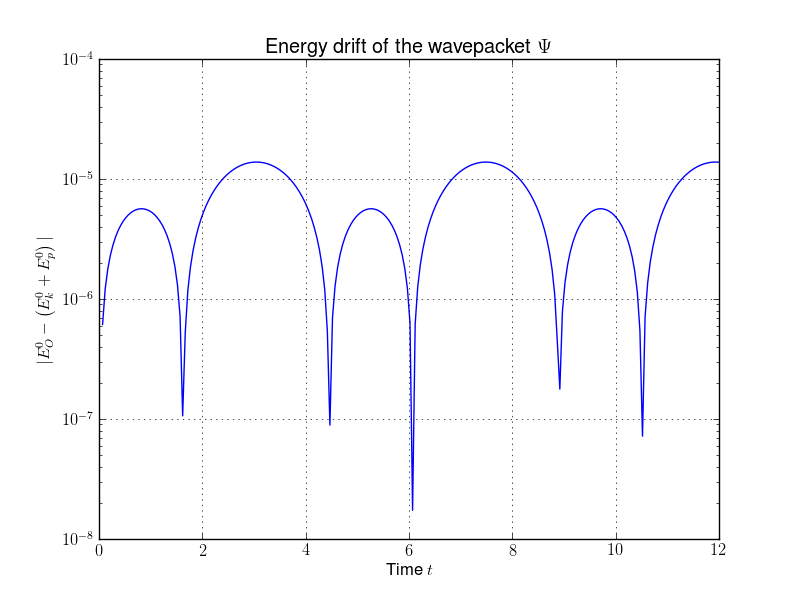
\includegraphics[width=0.5\linewidth]{./results/HO/energy_drift_block0_log.png}
  } \\
  \caption[Energies of a wavepacket in an harmonic oscillator]
          {The kinetic, potential and total energy and the drift of the
           total energy of a wavepacket in a two-dimensional harmonic oscillator.
    \subref{fig:ho_energies} The energies.
    \subref{fig:ho_energy_drift} The energy drift.
    \label{fig:ho_energy_plots}
  }
\end{figure}

\begin{figure}
  \centering
  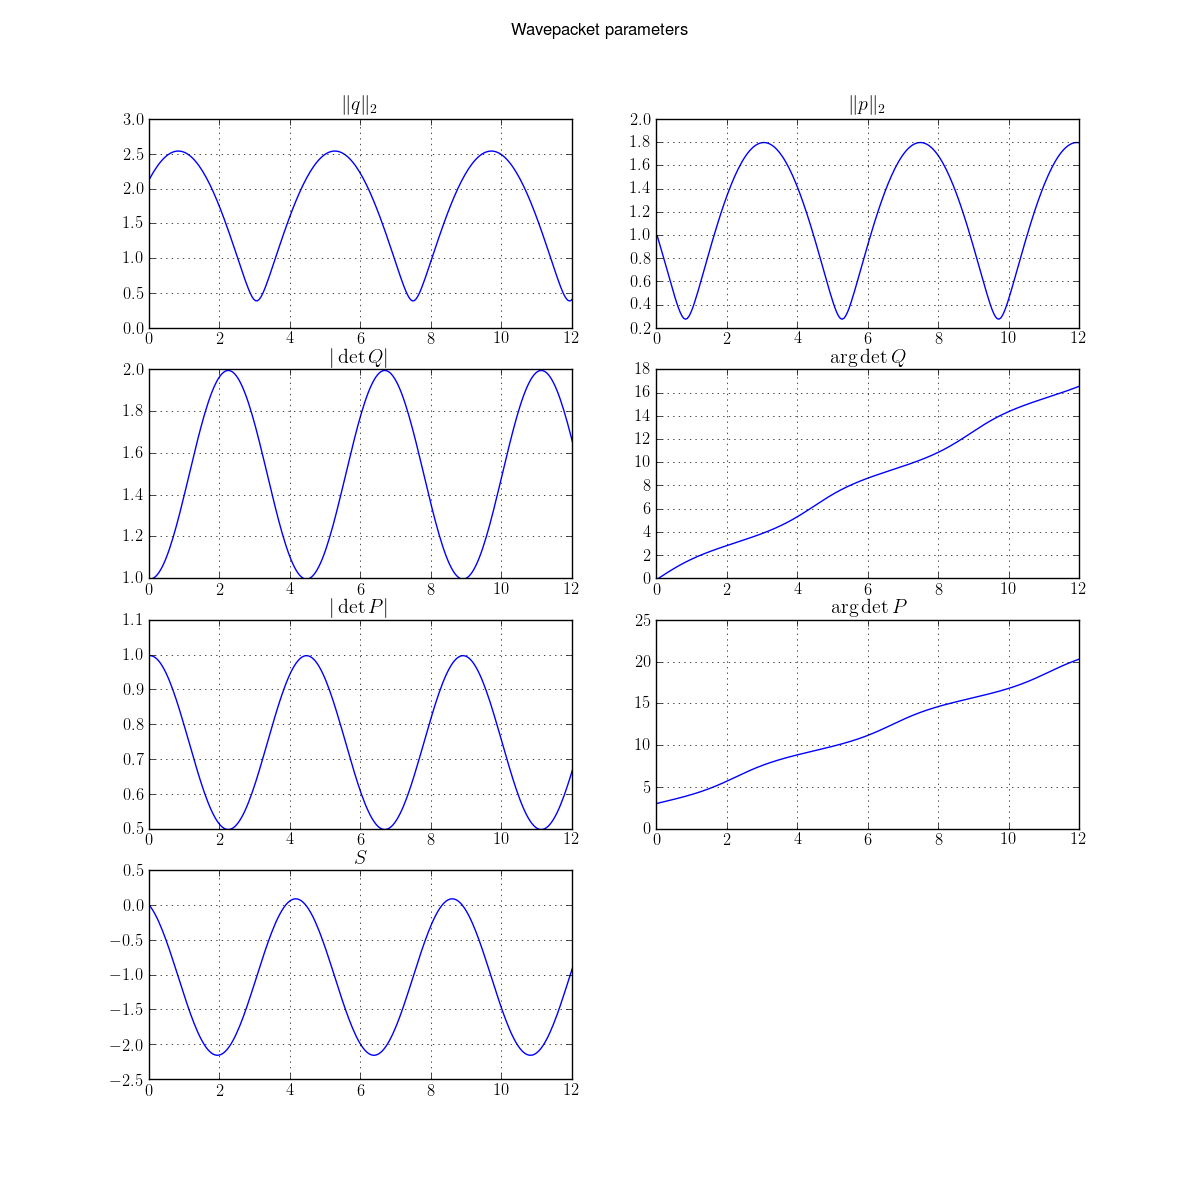
\includegraphics[width=\linewidth]{./results/HO/wavepacket_parameters_abs_ang_block0.png}
  \caption{Time-evolution of the parameter set $\Pi$ of a wavepacket in a
           two-dimensional harmonic oscillator.}
  \label{fig:ho_parameters}
\end{figure}

\begin{figure}
  \centering
  \subfloat[][]{
    \label{fig:ho_traject_q}
    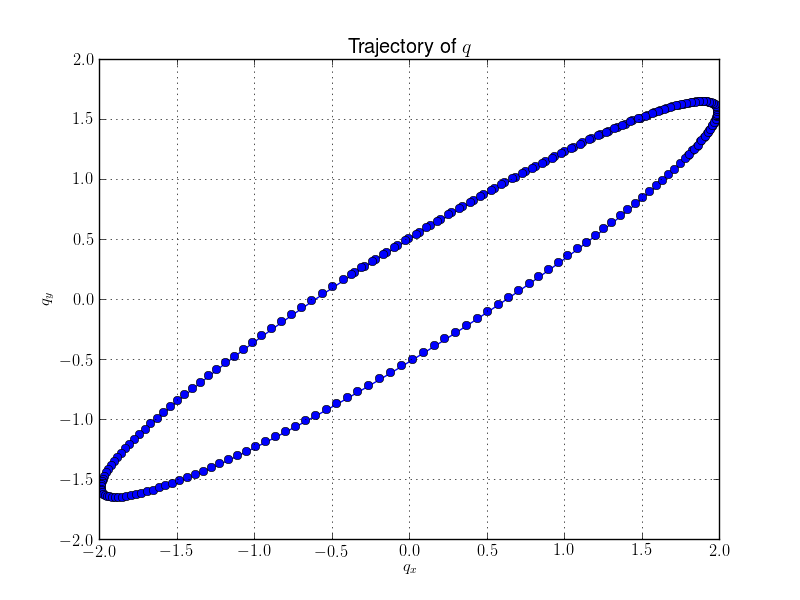
\includegraphics[width=0.5\linewidth]{./results/HO/wavepacket_parameters_trajectoryq_block0.png}
  }
  \subfloat[][]{
    \label{fig:ho_traject_p}
    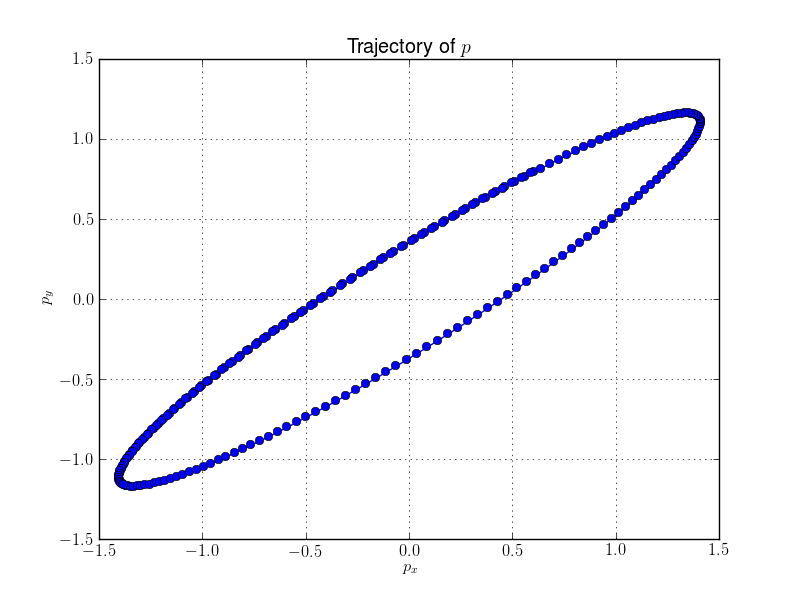
\includegraphics[width=0.5\linewidth]{./results/HO/wavepacket_parameters_trajectoryp_block0.png}
  } \\
  \caption[Trajectories of the position and momentum parameters]{
    Trajectories of the parameters $\vec{q}$ and $\vec{p}$.
    \subref{fig:ho_traject_q} Trajectory of $\vec{q}$.
    \subref{fig:ho_traject_p} Trajectory of $\vec{p}$.
    \label{fig:ho_traject_qp}
  }
\end{figure}

\begin{figure}
  \centering
  \subfloat[][]{
    \label{fig:ho_traject_Q}
    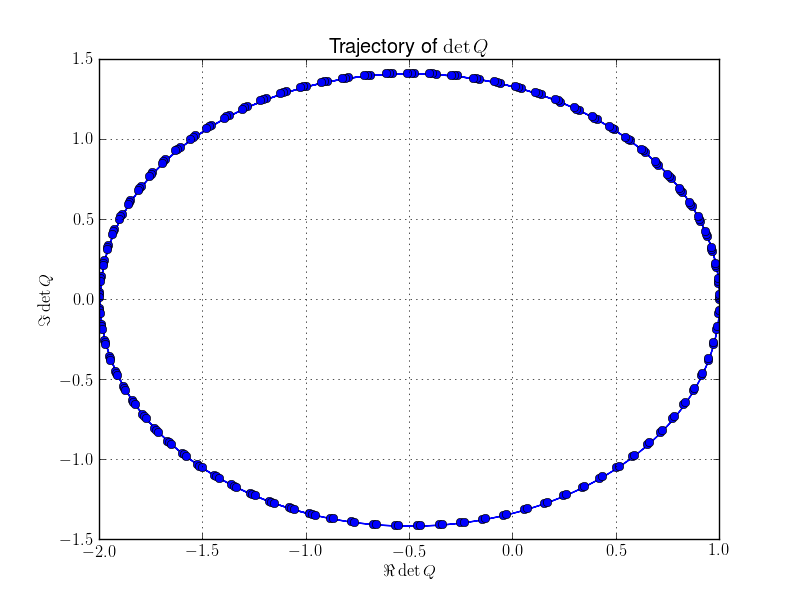
\includegraphics[width=0.5\linewidth]{./results/HO/wavepacket_parameters_trajectoryQ_block0.png}
  }
  \subfloat[][]{
    \label{fig:ho_traject_P}
    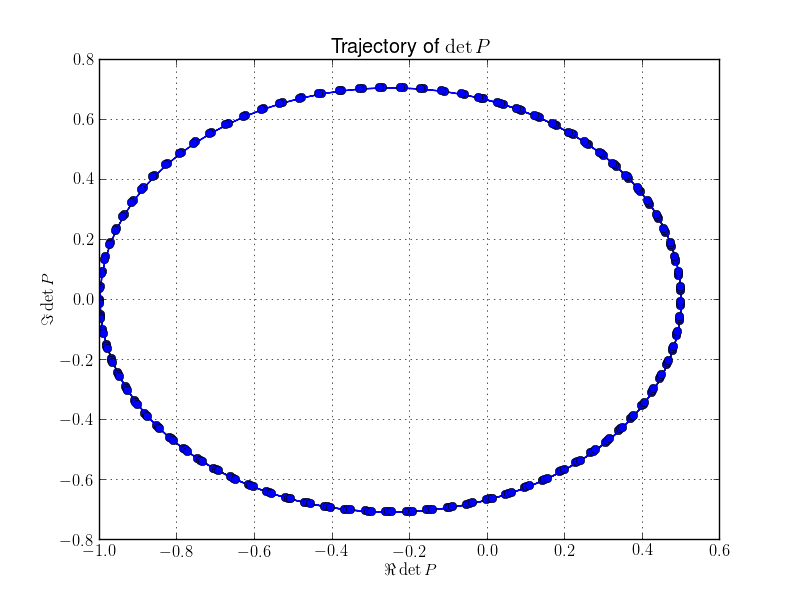
\includegraphics[width=0.5\linewidth]{./results/HO/wavepacket_parameters_trajectoryP_block0.png}
  } \\
  \caption[Trajectories of the spread matrices]{
    Trajectories of $\det\mat{Q}$ and $\det\mat{P}$ in the complex plane.
    \subref{fig:ho_traject_Q} Trajectory of $\det\mat{Q}$.
    \subref{fig:ho_traject_P} Trajectory of $\det\mat{P}$.
    \label{fig:ho_traject_QP}
  }
\end{figure}

Another trivial but nice example is the combination of a free particle potential
with a harmonic oscillator. The potential is constant along one direction while
quadratic along the other, we get:

\begin{equation} \label{eq:harmonic_channel}
  V(x,y) \assign \frac{1}{4} y^2 \,.
\end{equation}

The following simulation results were obtained by starting with a Gaussian $\phi_0$
with parameters:

\begin{align*}
  \vec{q} = \begin{pmatrix}
              0 \\ 1
            \end{pmatrix}
  \quad
  \vec{p} = \begin{pmatrix}
              0 \\ 0
            \end{pmatrix}
  \quad
  \mat{Q} = \begin{pmatrix}
              1 & 0 \\ 0 & 1
            \end{pmatrix}
  \quad
  \mat{P} = \begin{pmatrix}
              i & 0 \\ 0 & i
            \end{pmatrix}
  \quad
  S = 0
\end{align*}

and $\varepsilon = 0.1$.

\begin{figure}
  \centering
  \subfloat[][]{
    \label{fig:hofp_energies}
    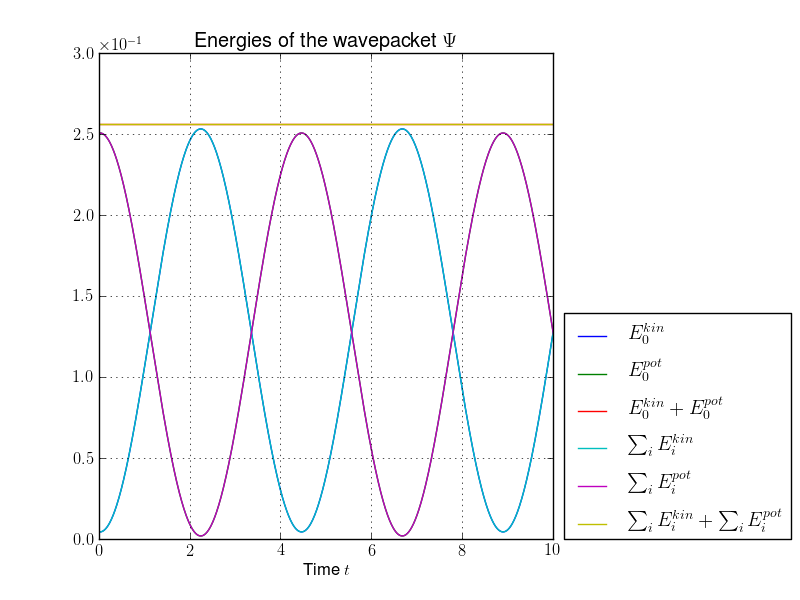
\includegraphics[width=0.5\linewidth]{./results/HO_FP/energies_block0.png}
  }
  \subfloat[][]{
    \label{fig:hofp_energy_drift}
    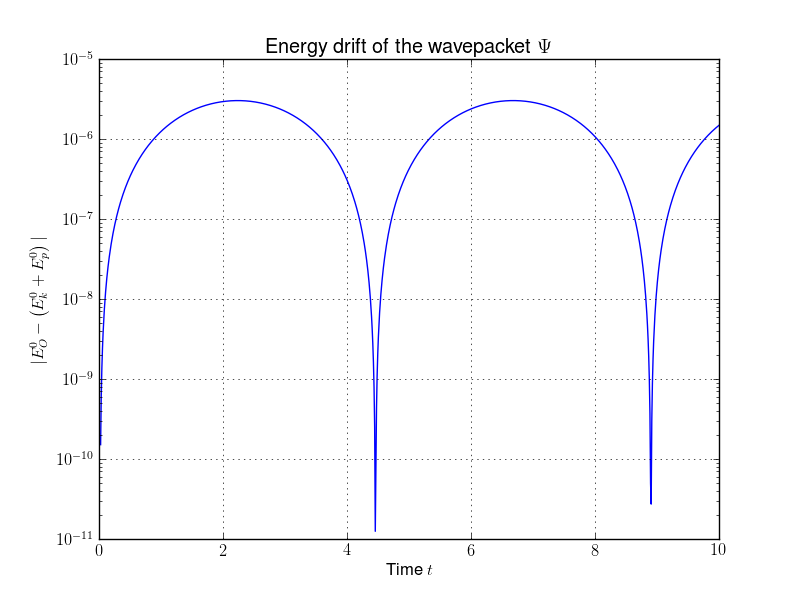
\includegraphics[width=0.5\linewidth]{./results/HO_FP/energy_drift_block0_log.png}
  } \\
  \caption[Energies of a wavepacket in a channel like oscillator]
          {The kinetic, potential and total energy and the drift of the
           total energy of a Gaussian wavepacket in the potential in \eqref{eq:harmonic_channel}.
    \subref{fig:hofp_energies} The energies.
    \subref{fig:hofp_energy_drift} The energy drift.
    \label{fig:hofp_energy_plots}
  }
\end{figure}

\begin{figure}
  \centering
  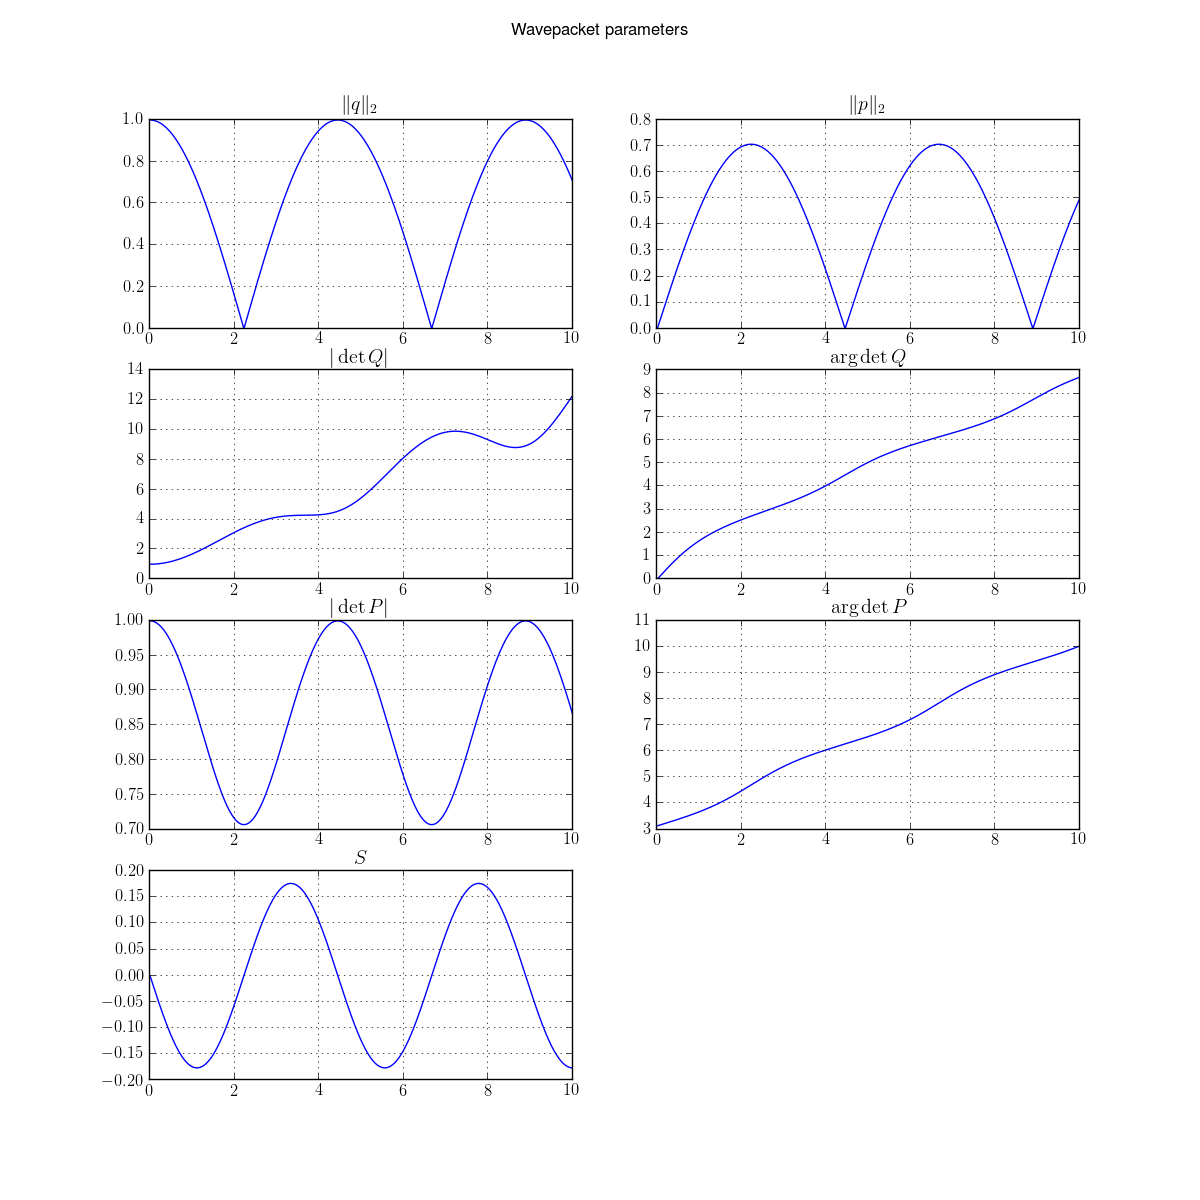
\includegraphics[width=\linewidth]{./results/HO_FP/wavepacket_parameters_abs_ang_block0.png}
  \caption{Time-evolution of the parameter set $\Pi$ of a Gaussian wavepacket in
           the potential in \eqref{eq:harmonic_channel}.}
  \label{fig:hofp_parameters}
\end{figure}

\begin{figure}
  \centering
  \subfloat[][]{
    \label{fig:hofp_traject_Q}
    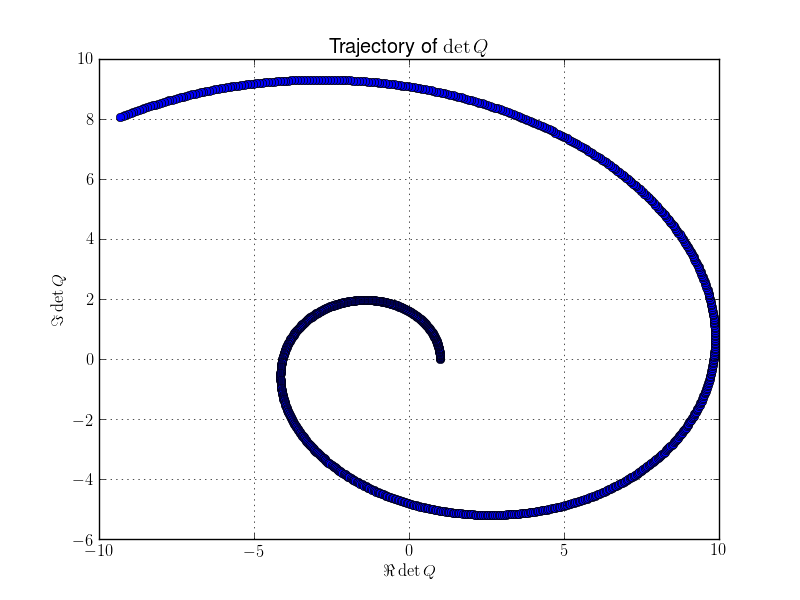
\includegraphics[width=0.5\linewidth]{./results/HO_FP/wavepacket_parameters_trajectoryQ_block0.png}
  }
  \subfloat[][]{
    \label{fig:hofp_traject_P}
    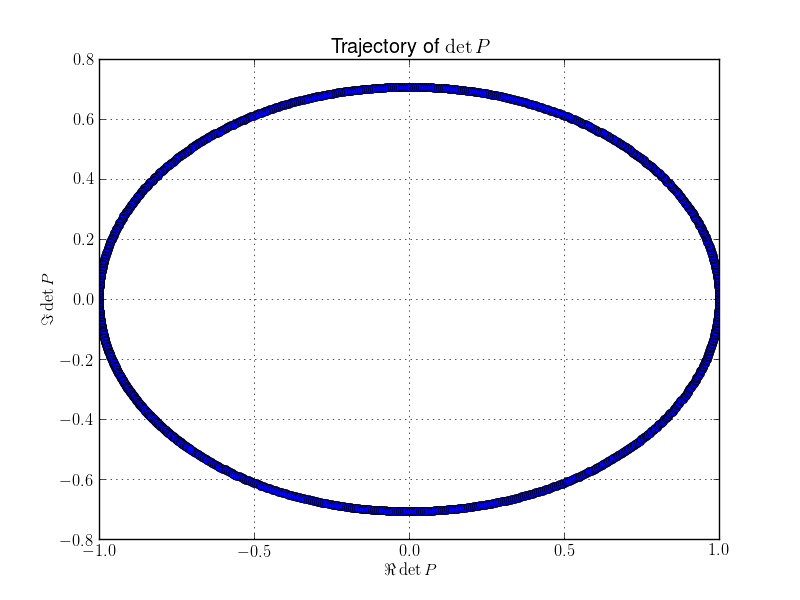
\includegraphics[width=0.5\linewidth]{./results/HO_FP/wavepacket_parameters_trajectoryP_block0.png}
  } \\
  \caption[Trajectories of the spread matrices]{
    Trajectories of $\det\mat{Q}$ and $\det\mat{P}$ in the complex plane.
    \subref{fig:hofp_traject_Q} Trajectory of $\det\mat{Q}$.
    \subref{fig:hofp_traject_P} Trajectory of $\det\mat{P}$.
    \label{fig:hofp_traject_QP}
  }
\end{figure}

An interesting fact appears if we look at the two eigenvalues $\lambda_0$ and $\lambda_1$
of $\mat{Q}$. We see that one oscillates and the other grows ad infinitum. Figure
\ref{fig:hofp_ev_Q} shows plots of $\lambda_0(t)$ and $\lambda_1(t)$.

\begin{figure}
  \centering
  \subfloat[][]{
    \label{fig:hofp_ev_Q_reim}
    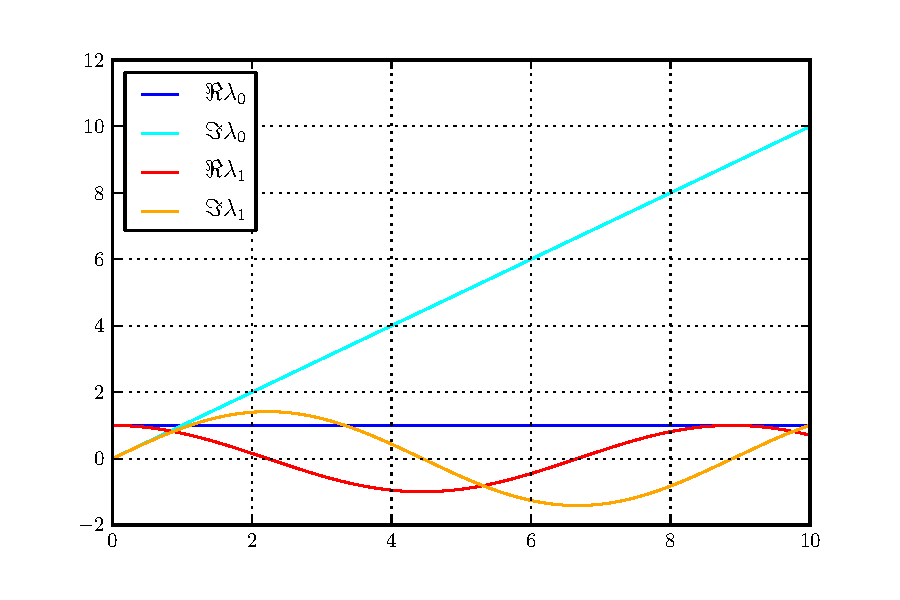
\includegraphics[width=0.5\linewidth]{./results/HO_FP/tube_reim_ev.pdf}
  }
  \subfloat[][]{
    \label{fig:hofp_ev_Q_abs}
    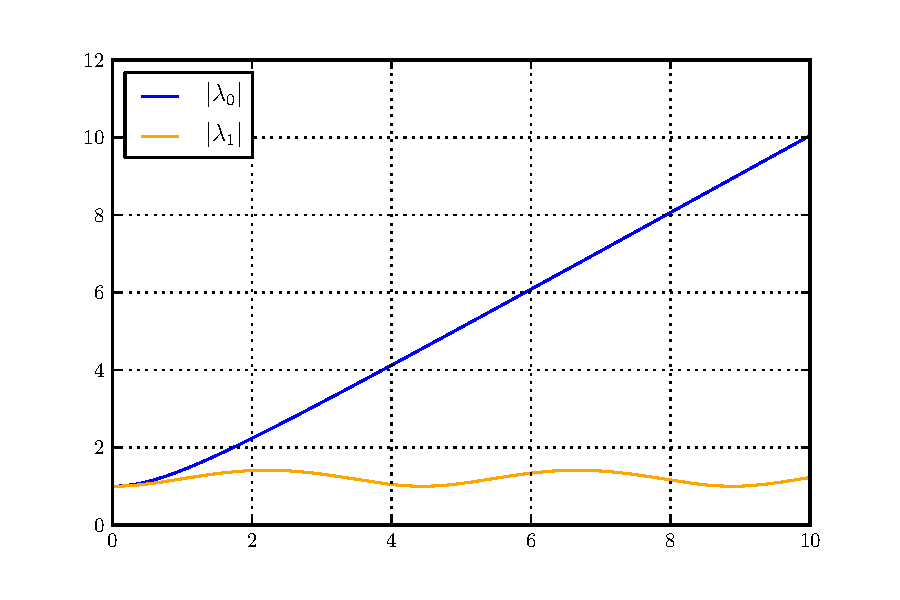
\includegraphics[width=0.5\linewidth]{./results/HO_FP/tube_abs_ev.pdf}
  } \\
  \caption[Eigenvalues of $Q$]{
    Time-evolution of the eigenvalues $\lambda_0$ and $\lambda_1$ of $\mat{Q}$.
    \subref{fig:hofp_ev_Q_reim} Real and imaginary parts.
    \subref{fig:hofp_ev_Q_abs} Absolute values.
    \label{fig:hofp_ev_Q}
  }
\end{figure}


\FloatBarrier
\section{Reproducing some other results}

We try to reproduce the results in section 5.1 of \cite{FGL_semiclassical_dynamics}.
The torsional potential in two dimensions is given by the expression:

\begin{equation}
  V(x,y) \assign (1-\cos(x)) + (1-\cos(y))
\end{equation}

and plotted in figure \ref{fig:torsional_potential}.

\begin{figure}
  \centering
  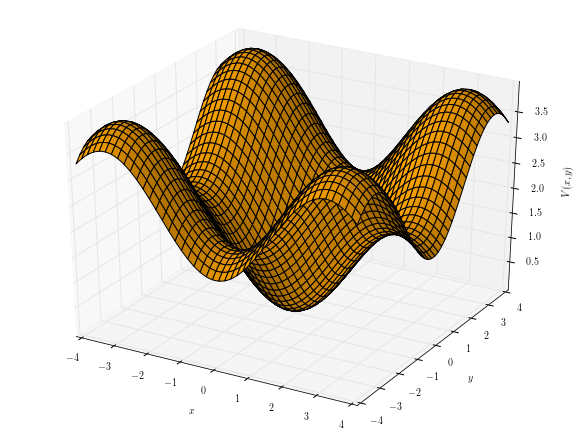
\includegraphics[scale=0.35]{./fig/torsional.png}
  \caption{The torsional potential in two dimensions.}
  \label{fig:torsional_potential}
\end{figure}

The initial parameter set $\Pi = \{\vec{q}, \vec{p}, \mat{Q}, \mat{P}, S\}$
for the wavepacket $\Psi = \phi_{0,0}$ is given as:

\begin{align*}
  \vec{q} = \begin{pmatrix}
              1 \\ 0
            \end{pmatrix}
  \quad
  \vec{p} = \begin{pmatrix}
              0 \\ 0
            \end{pmatrix}
  \quad
  \mat{Q} = \begin{pmatrix}
              1 & 0 \\ 0 & 1
            \end{pmatrix}
  \quad
  \mat{P} = \begin{pmatrix}
              i & 0 \\ 0 & i
            \end{pmatrix}
  \quad
  S = 0 \,.
\end{align*}

We use a hyperbolic cut basis shape $\mathfrak{K}$ with a cutoff value of $K=8$.
This yields 20 basis functions in total. For each simulation we use a time step
$\tau = 0.01$ and simulate until an end time of $T=20$. We perform three simulations
for different values of the semi-classical scaling parameter $\varepsilon$
\footnote{Note that we write $\varepsilon^2$ for what the authors of the paper call $\epsilon$.}.

\begin{figure}
  \centering
  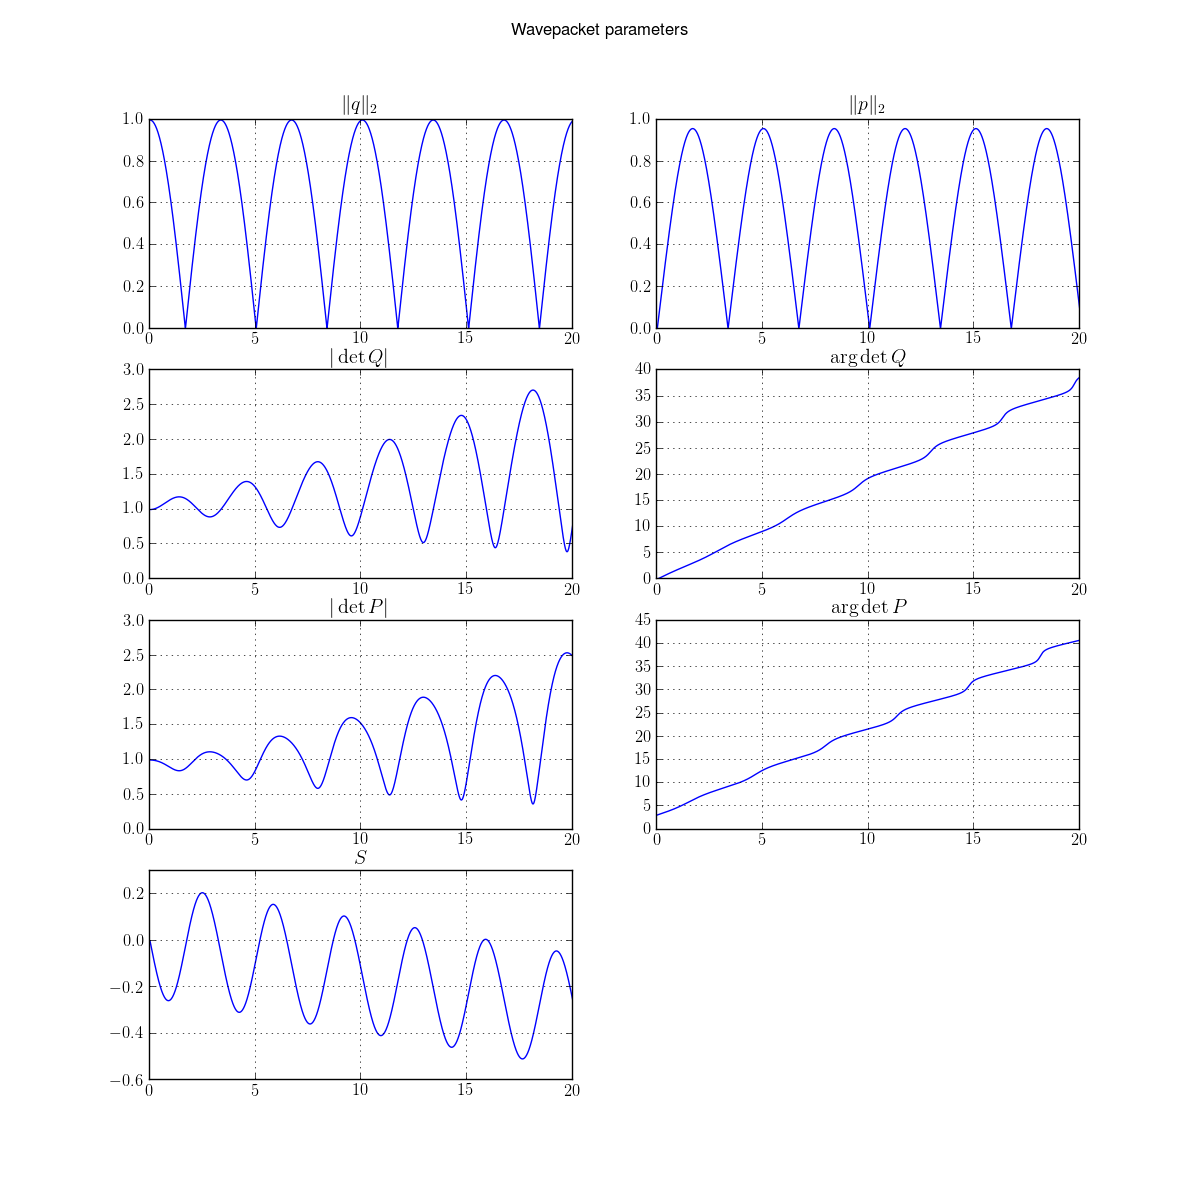
\includegraphics[width=\linewidth]{./results/config_cos_2_packets_case1/wavepacket_parameters_abs_ang_block0.png}
  \caption{Propagation of the parameter set $\Pi$. This is the same for all $\varepsilon$.}
  \label{fig:trosional_parameter_evolution}
\end{figure}

\begin{figure}
  \centering
  \subfloat[][]{
    \label{fig:torsional_case1_energies}
    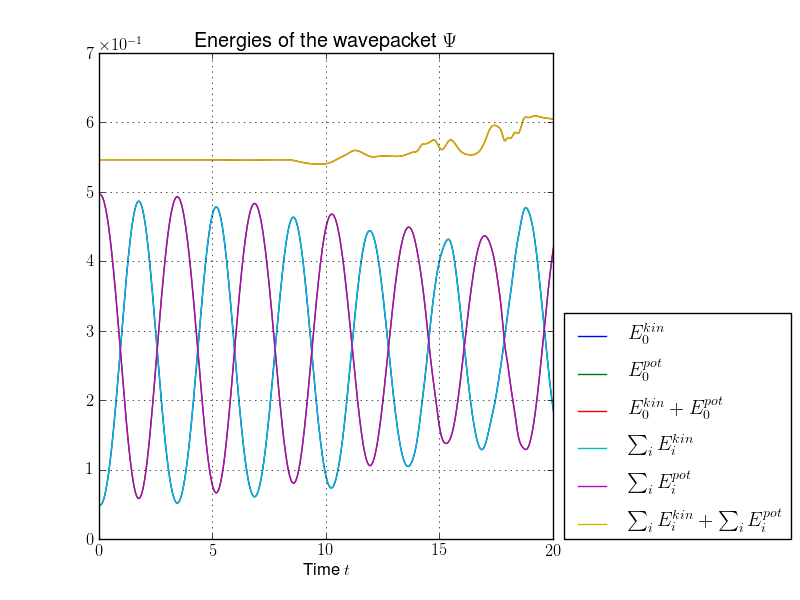
\includegraphics[width=0.5\linewidth]{./results/config_cos_2_packets_case1/energies_block0.png}
  }
  \subfloat[][]{
    \label{fig:torsional_case1_energy_drift}
    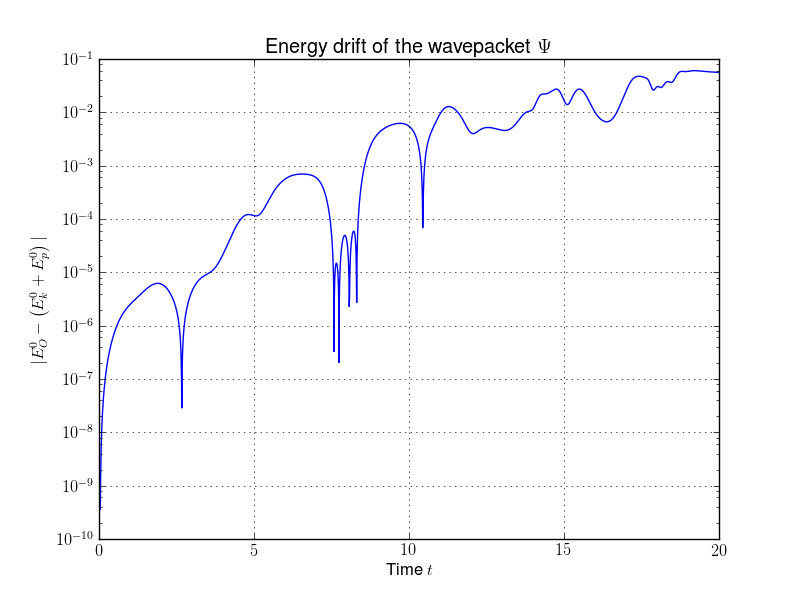
\includegraphics[width=0.5\linewidth]{./results/config_cos_2_packets_case1/energy_drift_block0_log.png}
  } \\
  \subfloat[][]{
    \label{fig:torsional_case2_energies}
    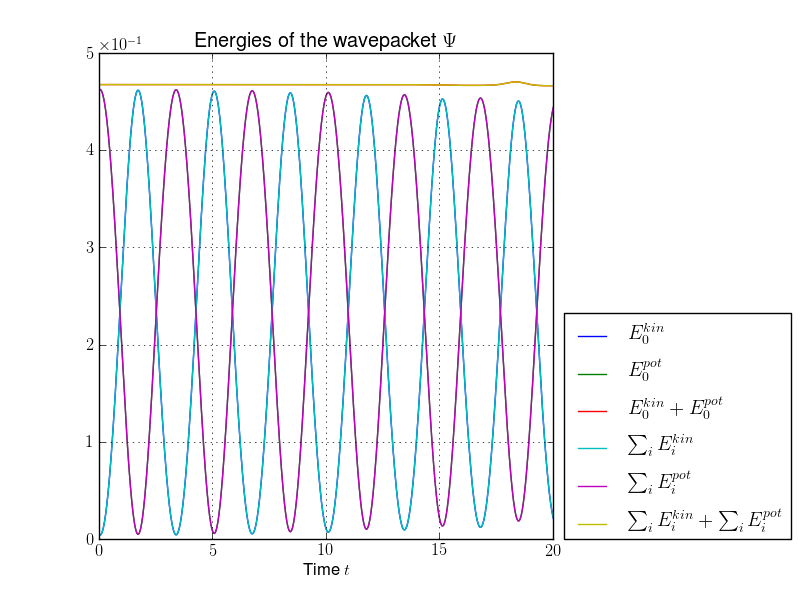
\includegraphics[width=0.5\linewidth]{./results/config_cos_2_packets_case2/energies_block0.png}
  }
  \subfloat[][]{
    \label{fig:torsional_case2_energy_drift}
    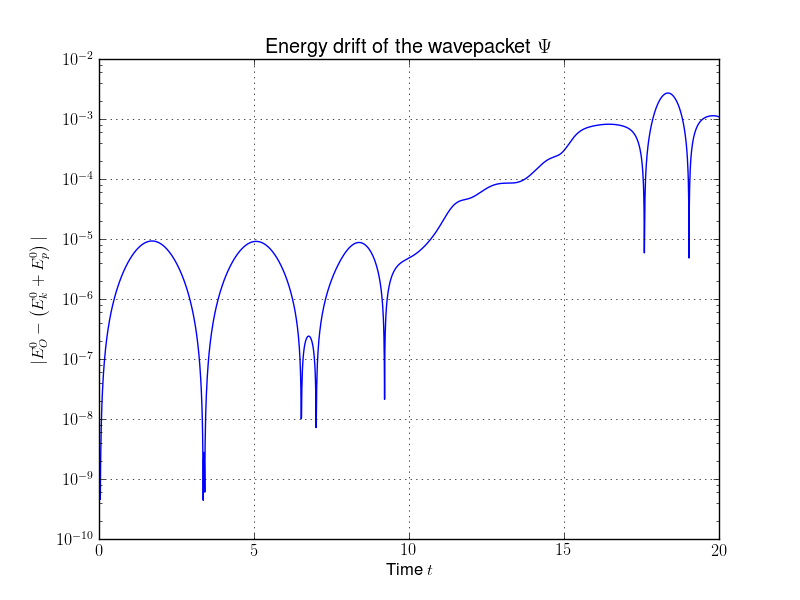
\includegraphics[width=0.5\linewidth]{./results/config_cos_2_packets_case2/energy_drift_block0_log.png}
  } \\
  \subfloat[][]{
    \label{fig:torsional_case3_energies}
    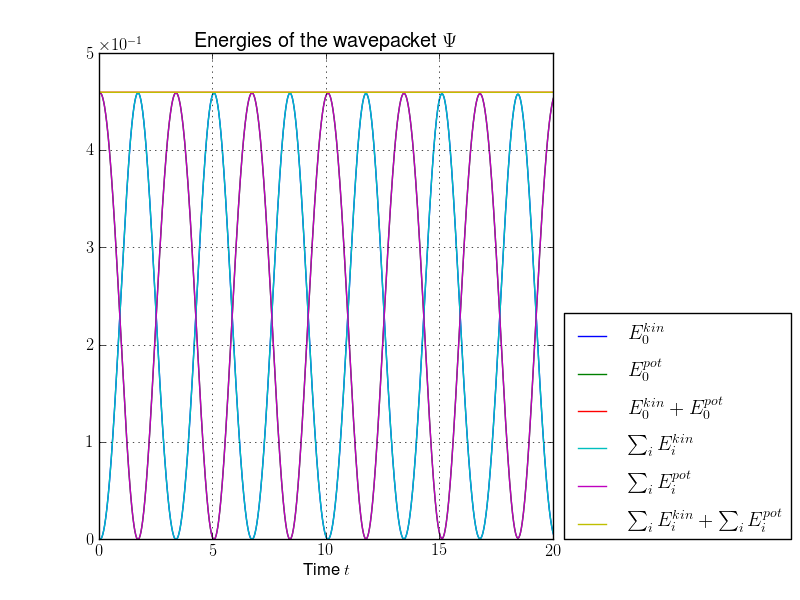
\includegraphics[width=0.5\linewidth]{./results/config_cos_2_packets_case3/energies_block0.png}
  }
  \subfloat[][]{
    \label{fig:torsional_case3_energy_drift}
    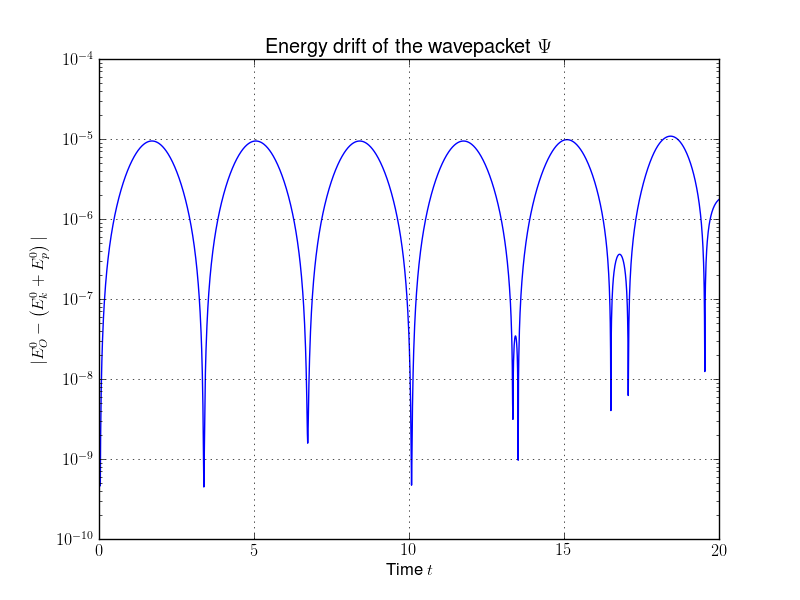
\includegraphics[width=0.5\linewidth]{./results/config_cos_2_packets_case3/energy_drift_block0_log.png}
  } \\
  \caption[Plots of the energies and drifts of a Gaussian in a torsional potential]{
    Plots of the kinetic, potential and total energy and the drift of the total energy
    of a Gaussian wavepacket in a 2D torsional potential. Note that despite of some violation of
    the total energy conservation we obtained perfect norm conservation (not shown here).
    A larger basis set would reduce the error.
    \subref{fig:torsional_case1_energies}, \subref{fig:torsional_case1_energy_drift}
    A wavepacket $\Ket{\Psi} = \phi_{0,0}$ with $\varepsilon = \sqrt{0.1}$.
    \subref{fig:torsional_case2_energies}, \subref{fig:torsional_case2_energy_drift}
    A wavepacket $\Ket{\Psi} = \phi_{0,0}$ with $\varepsilon = \sqrt{0.01}$.
    \subref{fig:torsional_case3_energies}, \subref{fig:torsional_case3_energy_drift}
    A wavepacket $\Ket{\Psi} = \phi_{0,0}$ with $\varepsilon = \sqrt{0.001}$.
%     \subref{fig:torsional_case1_energies} A wavepacket $\Ket{\Psi} = \phi_{0,0}$ with $\varepsilon = \sqrt{0.1}$.
%     \subref{fig:torsional_case1_energy_drift} A wavepacket $\Ket{\Psi} = \phi_{0,0}$ with $\varepsilon = \sqrt{0.1}$.
%     \subref{fig:torsional_case2_energies} A wavepacket $\Ket{\Psi} = \phi_{0,0}$ with $\varepsilon = \sqrt{0.01}$.
%     \subref{fig:torsional_case2_energy_drift} A wavepacket $\Ket{\Psi} = \phi_{0,0}$ with $\varepsilon = \sqrt{0.01}$.
%     \subref{fig:torsional_case3_energies} A wavepacket $\Ket{\Psi} = \phi_{0,0}$ with $\varepsilon = \sqrt{0.001}$.
%     \subref{fig:torsional_case3_energy_drift} A wavepacket $\Ket{\Psi} = \phi_{0,0}$ with $\varepsilon = \sqrt{0.001}$.
    \label{fig:torsional_energies}
  }
\end{figure}


\FloatBarrier
\section{A simple avoided crossing}

We generalise a model for a single avoided crossing of two energy levels.
The one-dimensional potential was studied in \cite{FGL_semiclassical_dynamics, B_bachelor_thesis}.
We extend this potential to two dimensions by making it rotationally symmetric. The equation
for $\mat{V}$ becomes:

\begin{equation} \label{eq:rotgap_avoided_crossing}
  \mat{V}(x,y) \assign
  \begin{pmatrix}
    \frac{1}{2} \tanh{\left(\sqrt{x^2 + y^2} \right)} & \delta \\
    \delta                                            & - \frac{1}{2} \tanh{\left(\sqrt{x^2 + y^2}\right)}
  \end{pmatrix}
\end{equation}

with $\delta$ being half of the energy level gap. The potential is shown in figure \ref{fig:rotgap_avoided_crossing}.

\begin{figure}[ht!]
  \centering
  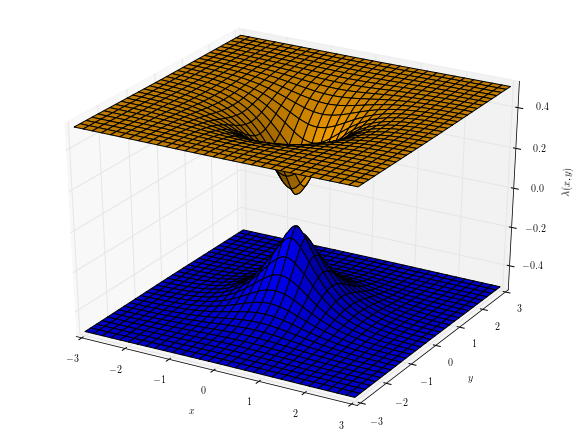
\includegraphics[width=0.7\linewidth]{./fig/delta_gap_rotsym.png}
  \caption{Energy levels of the avoided crossing given by equation \eqref{eq:rotgap_avoided_crossing}
          for $\delta = 0.08$.}
  \label{fig:rotgap_avoided_crossing}
\end{figure}

In the following simulation results we varied the value of $\varepsilon$ and the gap size $\delta$.
The initial parameter values are:

\begin{align*}
  \vec{q} = \begin{pmatrix}
              -3 \\ 0
            \end{pmatrix}
  \quad
  \vec{p} = \begin{pmatrix}
              0.5 \\ 0
            \end{pmatrix}
  \quad
  \mat{Q} = \begin{pmatrix}
              1 & 0 \\ 0 & 1
            \end{pmatrix}
  \quad
  \mat{P} = \begin{pmatrix}
              i & 0 \\ 0 & i
            \end{pmatrix}
  \quad
  S = 0 \,.
\end{align*}

The timestep was set to $\tau = 0.01$.


\begin{figure}
  \centering
  \subfloat[][]{
    \label{fig:dgr_16_0-01_0-01_e}
    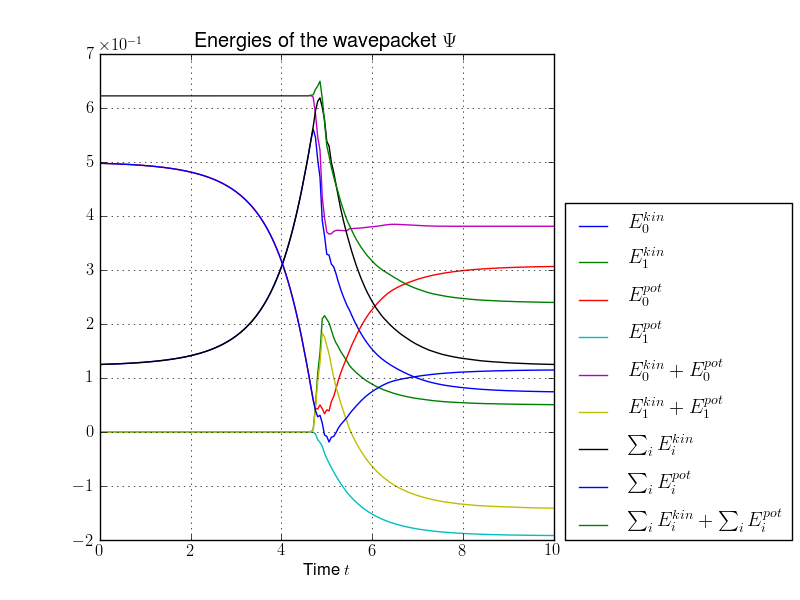
\includegraphics[width=0.5\linewidth]{./results/deltagap_rotsym/Parameters[bsize=16][eps=0-01][delta=0-01]/energies_block0.png}
  }
  \subfloat[][]{
    \label{fig:dgr_16_0-01_0-01_ed}
    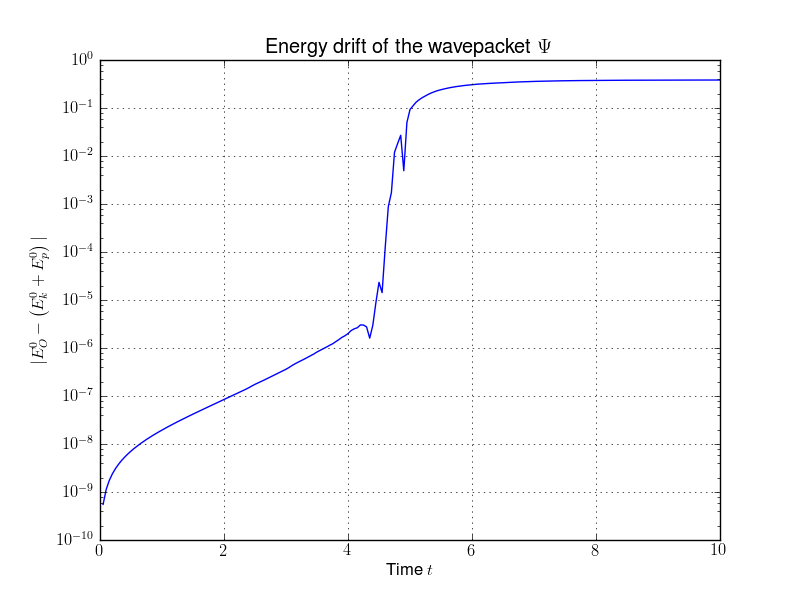
\includegraphics[width=0.5\linewidth]{./results/deltagap_rotsym/Parameters[bsize=16][eps=0-01][delta=0-01]/energy_drift_block0_log.png}
  } \\
  \subfloat[][]{
    \label{fig:dgr_16_0-01_0-05_e}
    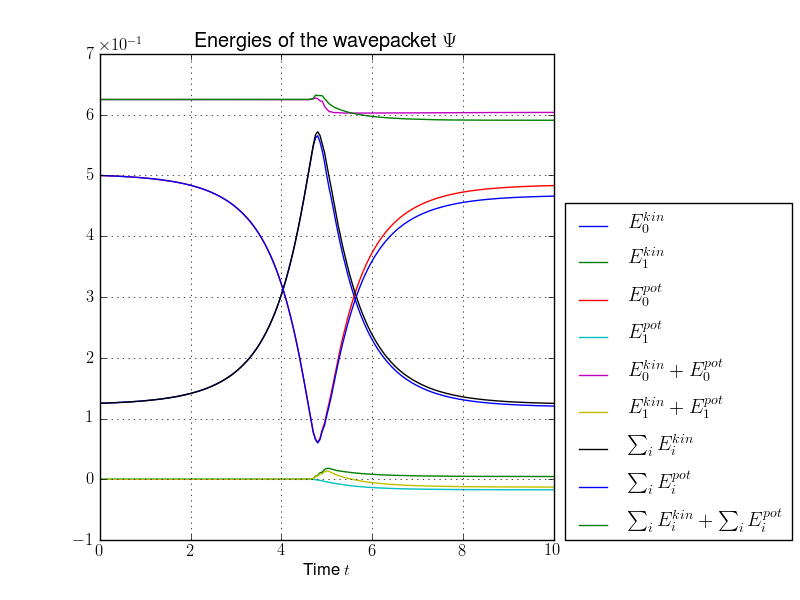
\includegraphics[width=0.5\linewidth]{./results/deltagap_rotsym/Parameters[bsize=16][eps=0-01][delta=0-05]/energies_block0.png}
  }
  \subfloat[][]{
    \label{fig:dgr_16_0-01_0-05_ed}
    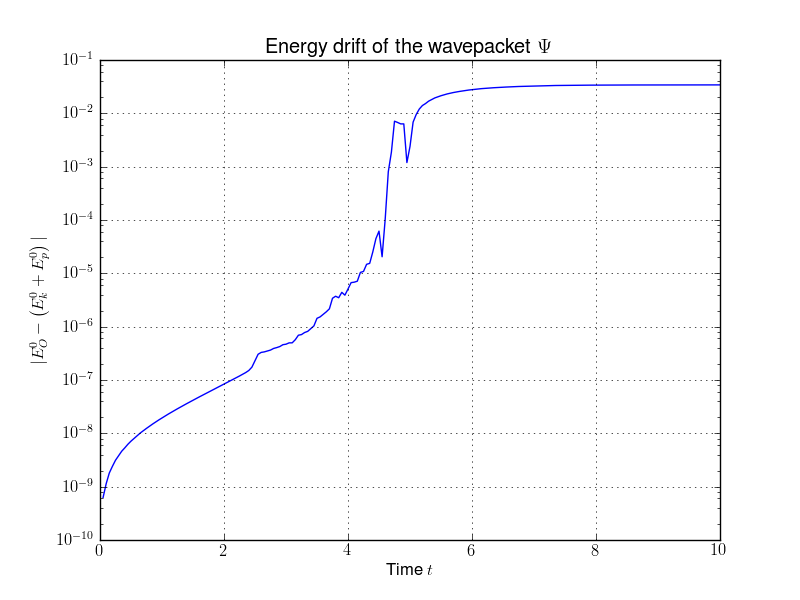
\includegraphics[width=0.5\linewidth]{./results/deltagap_rotsym/Parameters[bsize=16][eps=0-01][delta=0-05]/energy_drift_block0_log.png}
  } \\
  \subfloat[][]{
    \label{fig:dgr_16_0-01_0-1_e}
    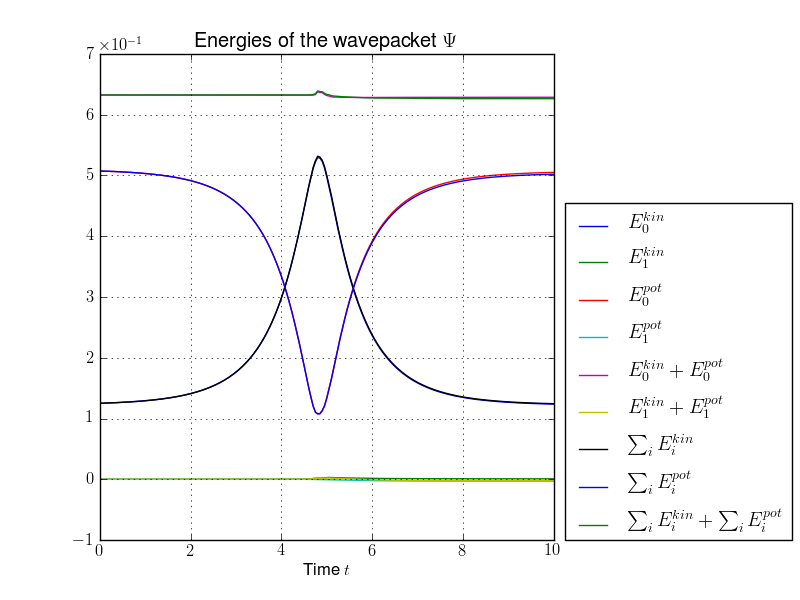
\includegraphics[width=0.5\linewidth]{./results/deltagap_rotsym/Parameters[bsize=16][eps=0-01][delta=0-1]/energies_block0.png}
  }
  \subfloat[][]{
    \label{fig:dgr_16_0-01_0-1_ed}
    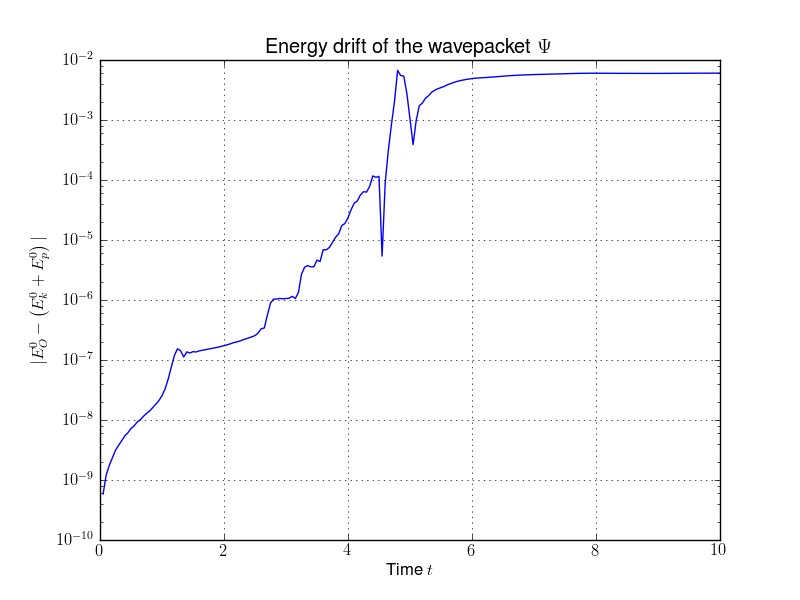
\includegraphics[width=0.5\linewidth]{./results/deltagap_rotsym/Parameters[bsize=16][eps=0-01][delta=0-1]/energy_drift_block0_log.png}
  } \\
  \caption[Plots of the energies and drifts for a simple avoided crossing]{
    Plots of the kinetic, potential and total energy and the drift of the total energy
    of a Gaussian wavepacket $\Ket{\Psi} = \phi_{0,0}$. The basis shape is a hyperbolic cut with cut-off $K = 16$
    and $\varepsilon = 0.01$. The simulations for $\delta = 0.01$ would need a larger
    basis to work properly.
    \subref{fig:dgr_16_0-01_0-01_e}, \subref{fig:dgr_16_0-01_0-01_ed} $\delta = 0.01$
    \subref{fig:dgr_16_0-01_0-05_e}, \subref{fig:dgr_16_0-01_0-05_ed} $\delta = 0.05$
    \subref{fig:dgr_16_0-01_0-1_e}, \subref{fig:dgr_16_0-01_0-1_ed} $\delta = 0.1$
%     \subref{fig:dgr_16_0-01_0-01_e} $\delta = 0.01$
%     \subref{fig:dgr_16_0-01_0-01_ed} $\delta = 0.01$
%     \subref{fig:dgr_16_0-01_0-05_e} $\delta = 0.05$
%     \subref{fig:dgr_16_0-01_0-05_ed} $\delta = 0.05$
%     \subref{fig:dgr_16_0-01_0-1_e} $\delta = 0.1$
%     \subref{fig:dgr_16_0-01_0-1_ed} $\delta = 0.1$
    \label{fig:deltagap_rotsym_16_energies_eps_001_part1}
  }
\end{figure}


\begin{figure}
  \centering
  \subfloat[][]{
    \label{fig:dgr_16_0-01_0-2_e}
    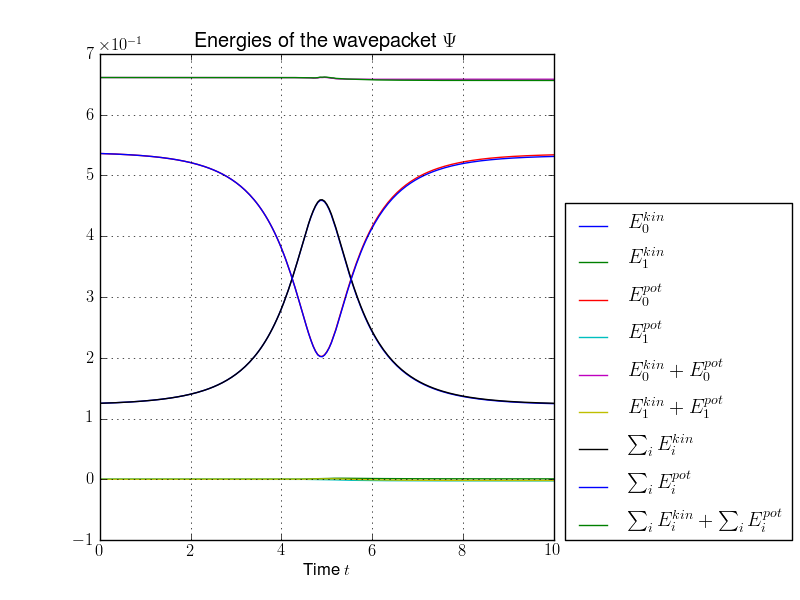
\includegraphics[width=0.5\linewidth]{./results/deltagap_rotsym/Parameters[bsize=16][eps=0-01][delta=0-2]/energies_block0.png}
  }
  \subfloat[][]{
    \label{fig:dgr_16_0-01_0-2_ed}
    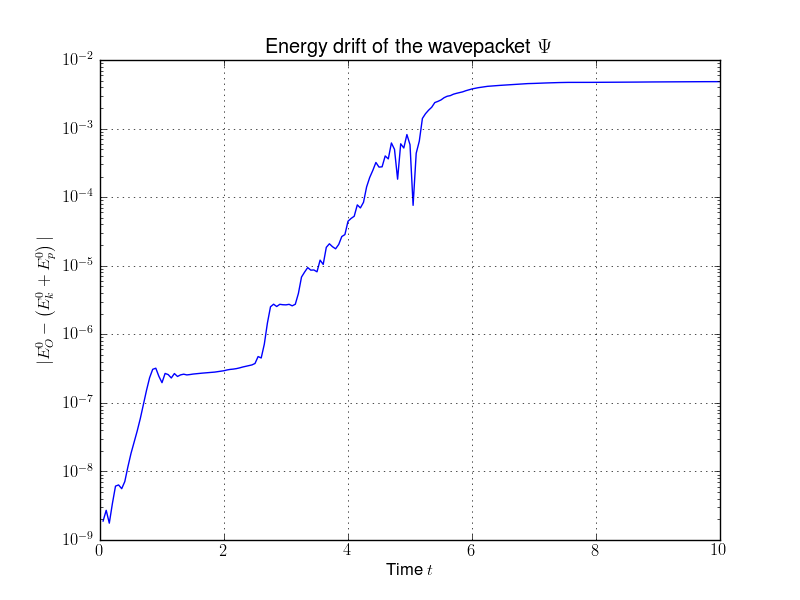
\includegraphics[width=0.5\linewidth]{./results/deltagap_rotsym/Parameters[bsize=16][eps=0-01][delta=0-2]/energy_drift_block0_log.png}
  } \\
  \subfloat[][]{
    \label{fig:dgr_16_0-01_0-5_e}
    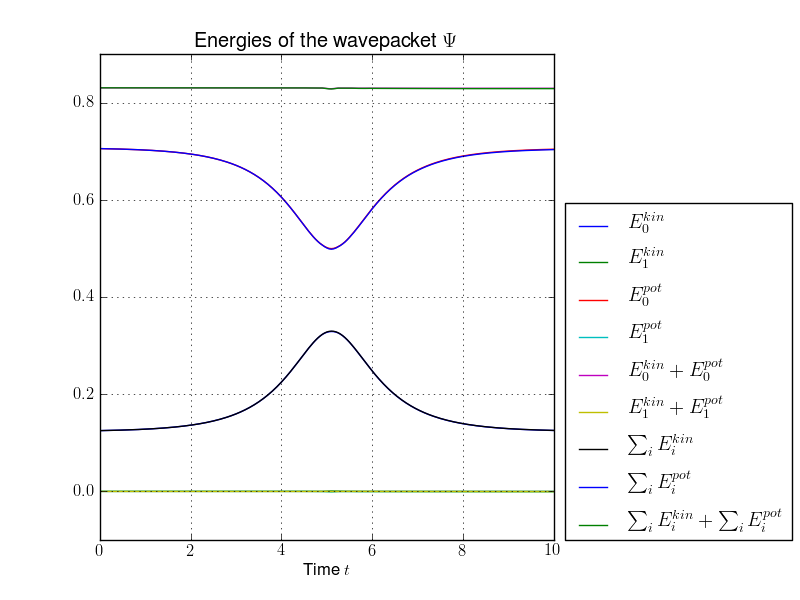
\includegraphics[width=0.5\linewidth]{./results/deltagap_rotsym/Parameters[bsize=16][eps=0-01][delta=0-5]/energies_block0.png}
  }
  \subfloat[][]{
    \label{fig:dgr_16_0-01_0-5_ed}
    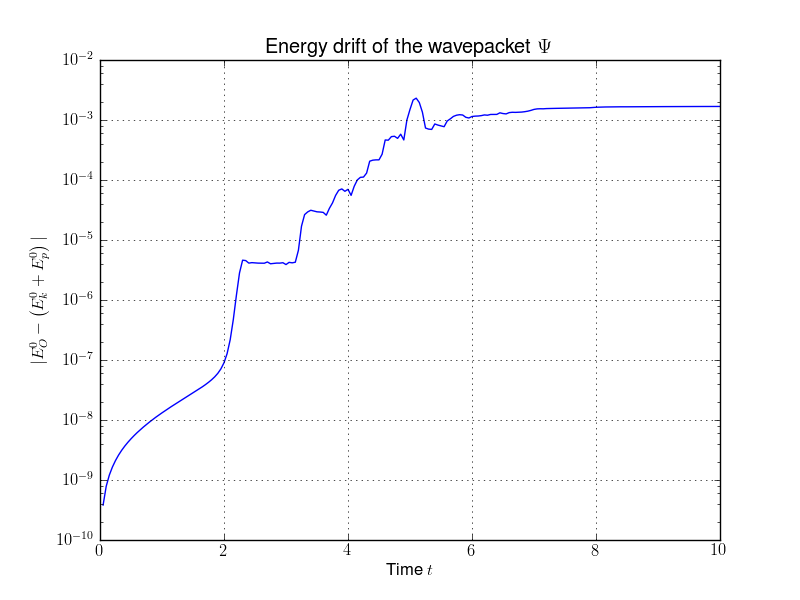
\includegraphics[width=0.5\linewidth]{./results/deltagap_rotsym/Parameters[bsize=16][eps=0-01][delta=0-5]/energy_drift_block0_log.png}
  } \\
  \subfloat[][]{
    \label{fig:dgr_16_0-01_1-0_e}
    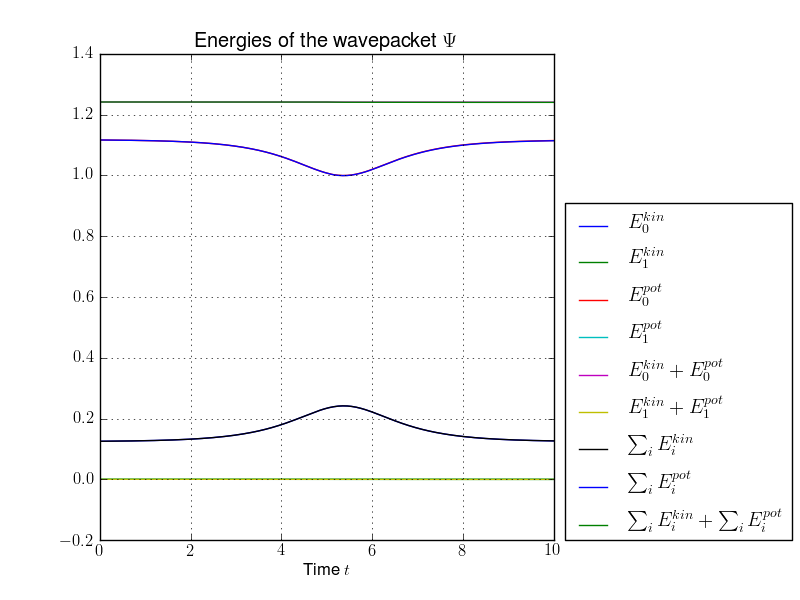
\includegraphics[width=0.5\linewidth]{./results/deltagap_rotsym/Parameters[bsize=16][eps=0-01][delta=1-0]/energies_block0.png}
  }
  \subfloat[][]{
    \label{fig:dgr_16_0-01_1-0_ed}
    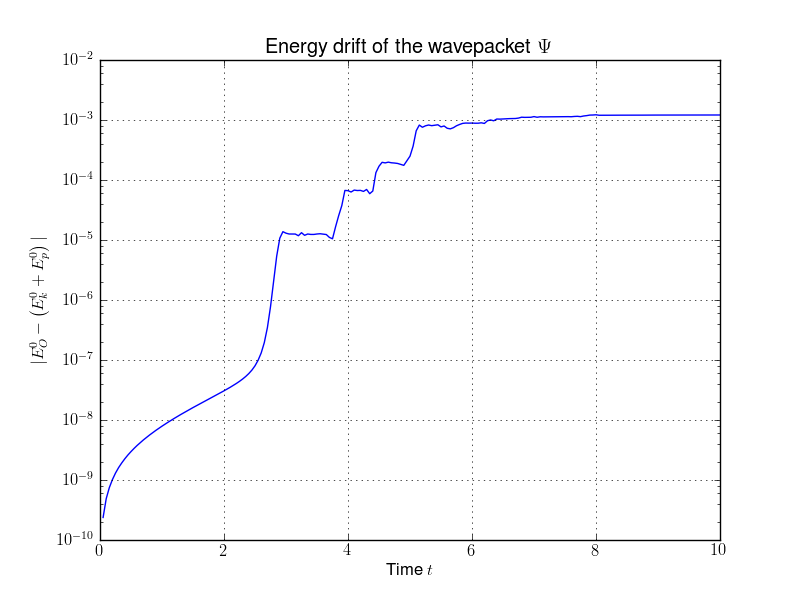
\includegraphics[width=0.5\linewidth]{./results/deltagap_rotsym/Parameters[bsize=16][eps=0-01][delta=1-0]/energy_drift_block0_log.png}
  } \\
  \caption[Plots of the energies and drifts for a simple avoided crossing]{
    Plots of the kinetic, potential and total energy and the drift of the total energy
    of a Gaussian wavepacket $\Ket{\Psi} = \phi_{0,0}$. The basis shape is a hyperbolic cut with cut-off $K = 16$
    and $\varepsilon = 0.01$.
    \subref{fig:dgr_16_0-01_0-2_e}, \subref{fig:dgr_16_0-01_0-2_ed} $\delta = 0.2$
    \subref{fig:dgr_16_0-01_0-5_e}, \subref{fig:dgr_16_0-01_0-5_ed} $\delta = 0.5$
    \subref{fig:dgr_16_0-01_1-0_e}, \subref{fig:dgr_16_0-01_1-0_ed} $\delta = 1.0$
%     \subref{fig:dgr_16_0-01_0-2_e} $\delta = 0.2$
%     \subref{fig:dgr_16_0-01_0-2_ed} $\delta = 0.2$
%     \subref{fig:dgr_16_0-01_0-5_e} $\delta = 0.5$
%     \subref{fig:dgr_16_0-01_0-5_ed} $\delta = 0.5$
%     \subref{fig:dgr_16_0-01_1-0_e} $\delta = 1.0$
%     \subref{fig:dgr_16_0-01_1-0_ed} $\delta = 1.0$
    \label{fig:deltagap_rotsym_16_energies_eps_001_part2}
  }
\end{figure}


\begin{figure}
  \centering
  \subfloat[][]{
    \label{fig:dgr_16_0-01_0-01_n}
    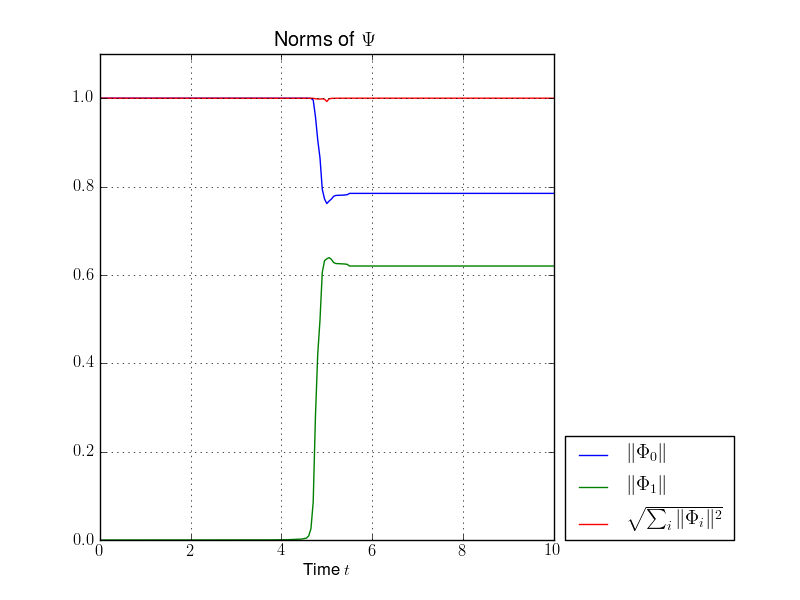
\includegraphics[width=0.5\linewidth]{./results/deltagap_rotsym/Parameters[bsize=16][eps=0-01][delta=0-01]/norms_block0.png}
  }
  \subfloat[][]{
    \label{fig:dgr_16_0-01_0-01_nd}
    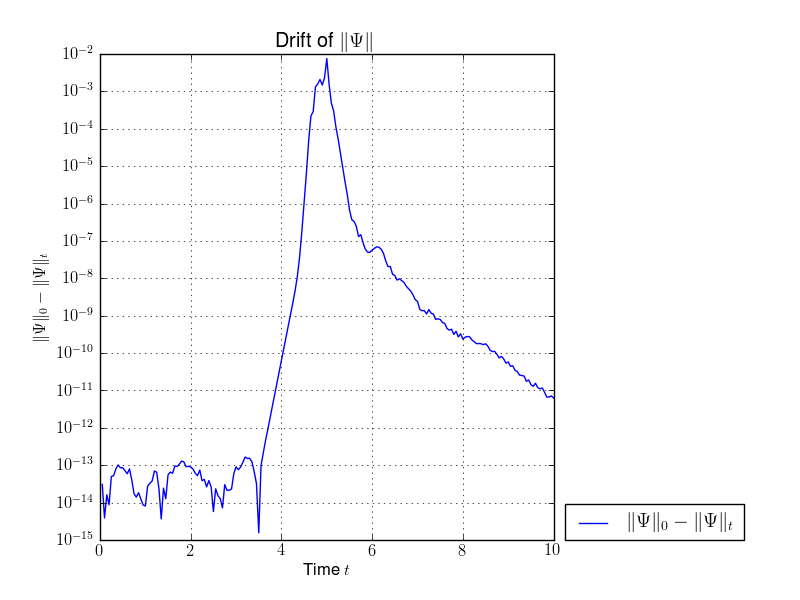
\includegraphics[width=0.5\linewidth]{./results/deltagap_rotsym/Parameters[bsize=16][eps=0-01][delta=0-01]/norms_drift_block0_log.png}
  } \\
  \subfloat[][]{
    \label{fig:dgr_16_0-01_0-05_n}
    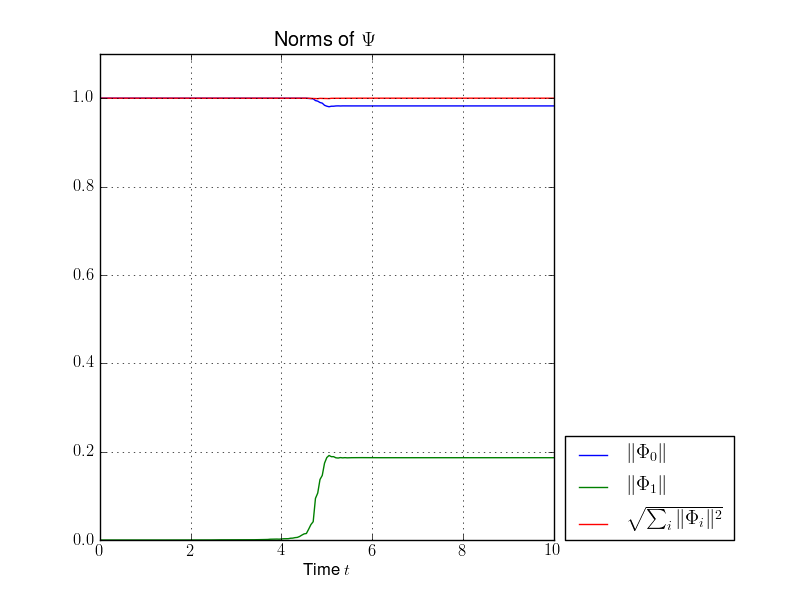
\includegraphics[width=0.5\linewidth]{./results/deltagap_rotsym/Parameters[bsize=16][eps=0-01][delta=0-05]/norms_block0.png}
  }
  \subfloat[][]{
    \label{fig:dgr_16_0-01_0-05_nd}
    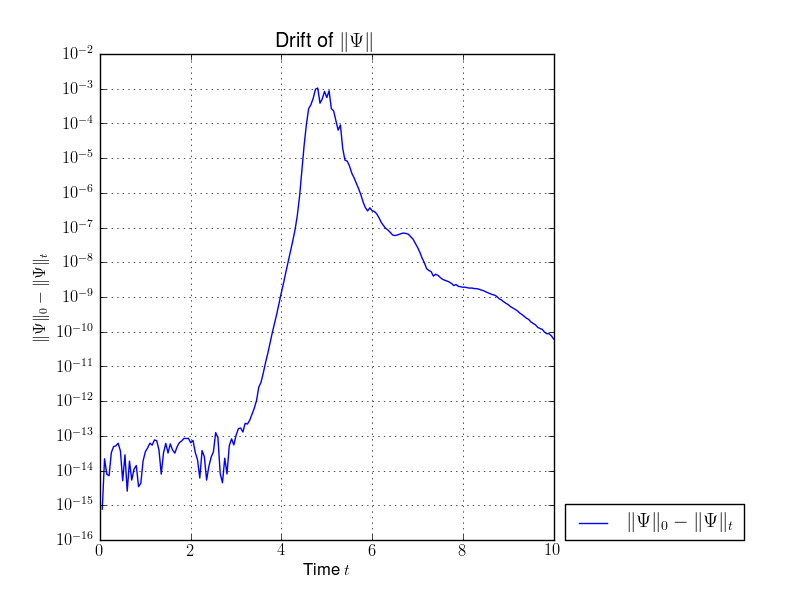
\includegraphics[width=0.5\linewidth]{./results/deltagap_rotsym/Parameters[bsize=16][eps=0-01][delta=0-05]/norms_drift_block0_log.png}
  } \\
  \subfloat[][]{
    \label{fig:dgr_16_0-01_0-1_n}
    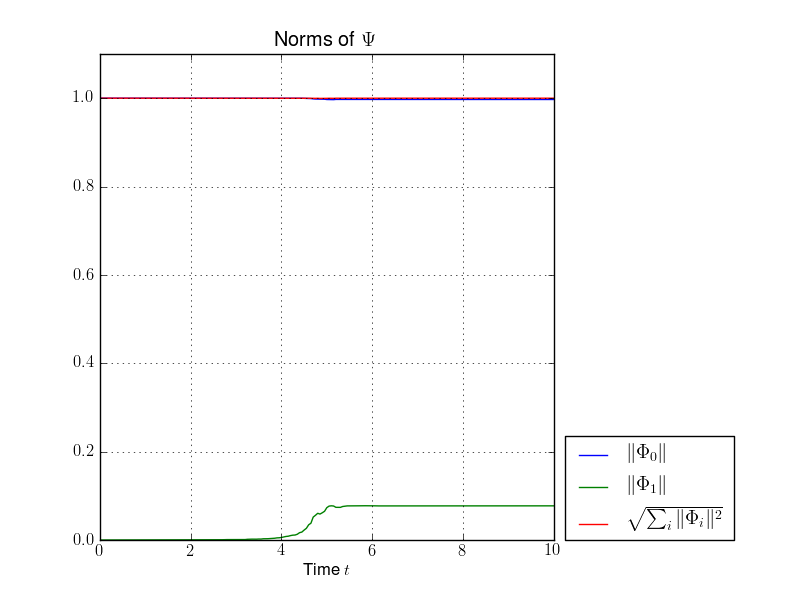
\includegraphics[width=0.5\linewidth]{./results/deltagap_rotsym/Parameters[bsize=16][eps=0-01][delta=0-1]/norms_block0.png}
  }
  \subfloat[][]{
    \label{fig:dgr_16_0-01_0-1_nd}
    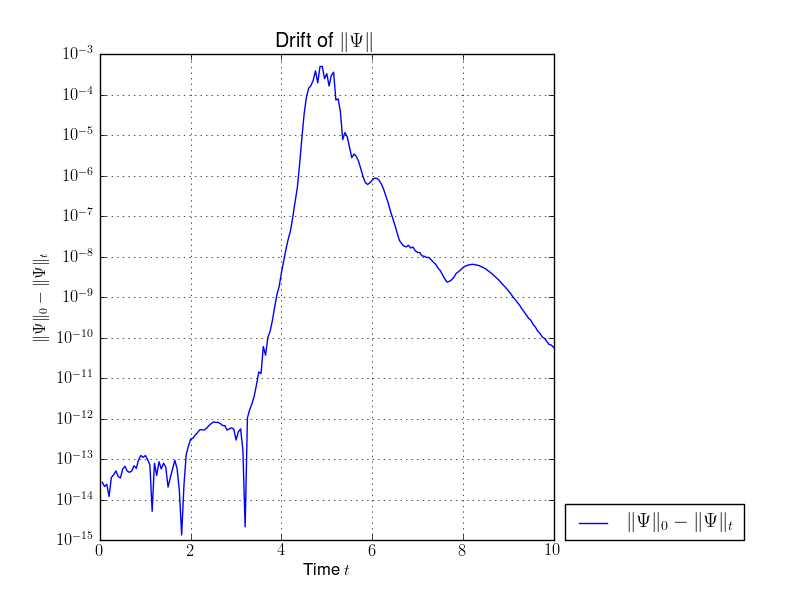
\includegraphics[width=0.5\linewidth]{./results/deltagap_rotsym/Parameters[bsize=16][eps=0-01][delta=0-1]/norms_drift_block0_log.png}
  } \\
  \caption[Plots of the norms and drifts for a simple avoided crossing]{
    Plots of the norm of the components on the upper and lower level and the drift of the total norm
    of a Gaussian wavepacket $\Ket{\Psi} = \phi_{0,0}$. The basis shape is a hyperbolic cut with cut-off $K = 16$
    and $\varepsilon = 0.01$.
    \subref{fig:dgr_16_0-01_0-01_n}, \subref{fig:dgr_16_0-01_0-01_nd} $\delta = 0.01$
    \subref{fig:dgr_16_0-01_0-05_n}, \subref{fig:dgr_16_0-01_0-05_nd} $\delta = 0.05$
    \subref{fig:dgr_16_0-01_0-1_n}, \subref{fig:dgr_16_0-01_0-1_nd} $\delta = 0.1$
%     \subref{fig:dgr_16_0-01_0-01_n} $\delta = 0.01$
%     \subref{fig:dgr_16_0-01_0-01_nd} $\delta = 0.01$
%     \subref{fig:dgr_16_0-01_0-05_n} $\delta = 0.05$
%     \subref{fig:dgr_16_0-01_0-05_nd} $\delta = 0.05$
%     \subref{fig:dgr_16_0-01_0-1_n} $\delta = 0.1$
%     \subref{fig:dgr_16_0-01_0-1_nd} $\delta = 0.1$
    \label{fig:deltagap_rotsym_16_norms_eps_001_part1}
  }
\end{figure}


\begin{figure}
  \centering
  \subfloat[][]{
    \label{fig:dgr_16_0-01_0-2_n}
    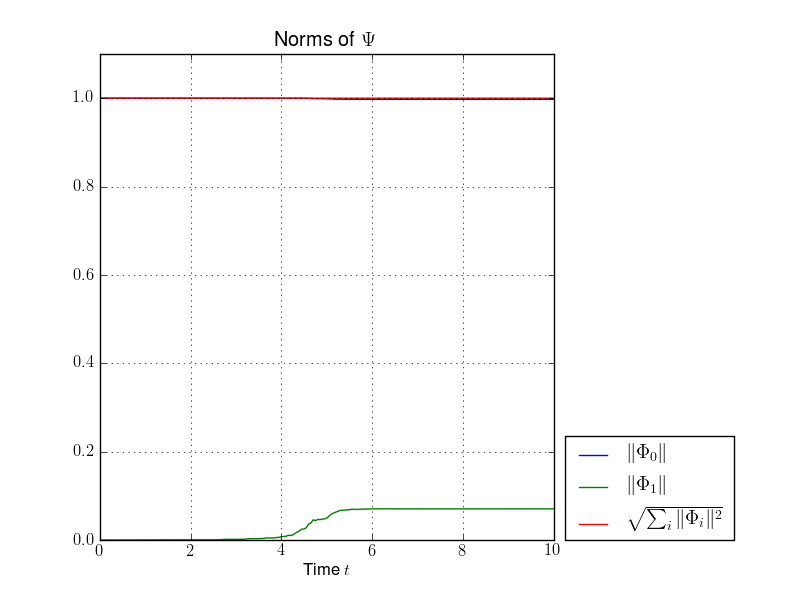
\includegraphics[width=0.5\linewidth]{./results/deltagap_rotsym/Parameters[bsize=16][eps=0-01][delta=0-2]/norms_block0.png}
  }
  \subfloat[][]{
    \label{fig:dgr_16_0-01_0-2_nd}
    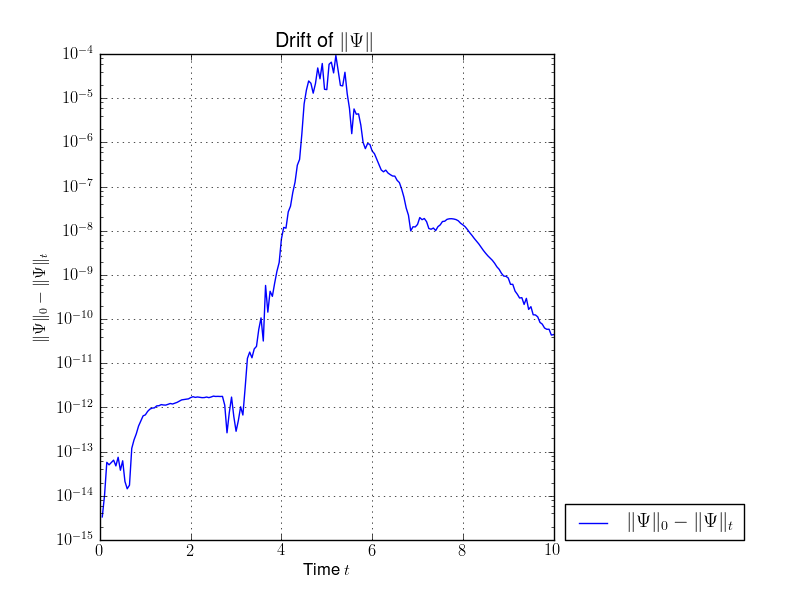
\includegraphics[width=0.5\linewidth]{./results/deltagap_rotsym/Parameters[bsize=16][eps=0-01][delta=0-2]/norms_drift_block0_log.png}
  } \\
  \subfloat[][]{
    \label{fig:dgr_16_0-01_0-5_n}
    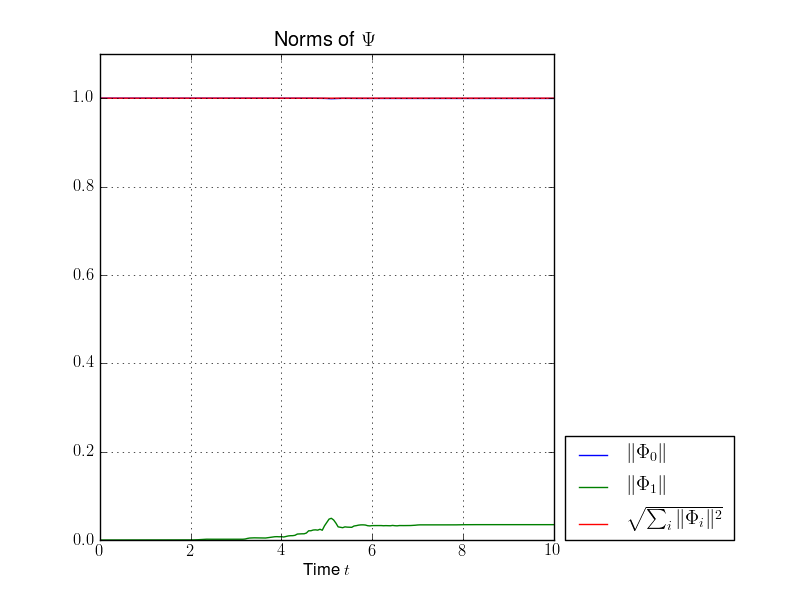
\includegraphics[width=0.5\linewidth]{./results/deltagap_rotsym/Parameters[bsize=16][eps=0-01][delta=0-5]/norms_block0.png}
  }
  \subfloat[][]{
    \label{fig:dgr_16_0-01_0-5_nd}
    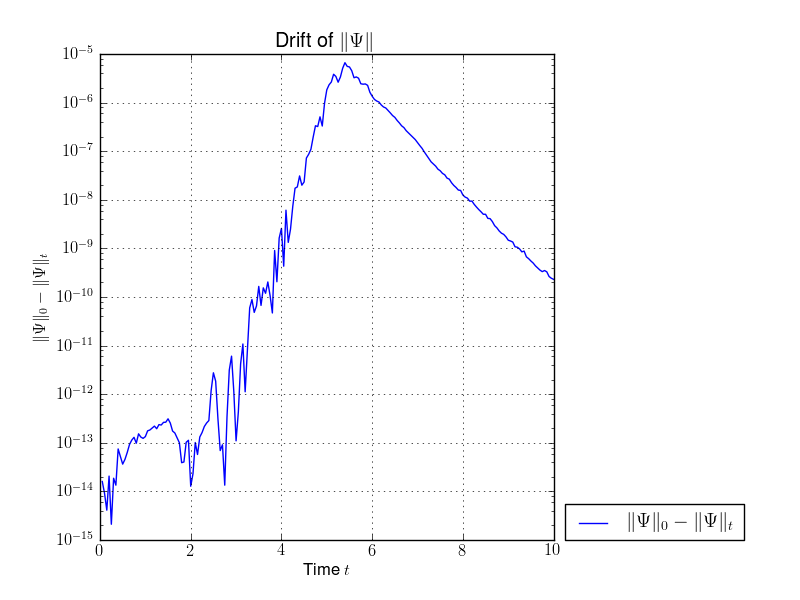
\includegraphics[width=0.5\linewidth]{./results/deltagap_rotsym/Parameters[bsize=16][eps=0-01][delta=0-5]/norms_drift_block0_log.png}
  } \\
  \subfloat[][]{
    \label{fig:dgr_16_0-01_1-0_n}
    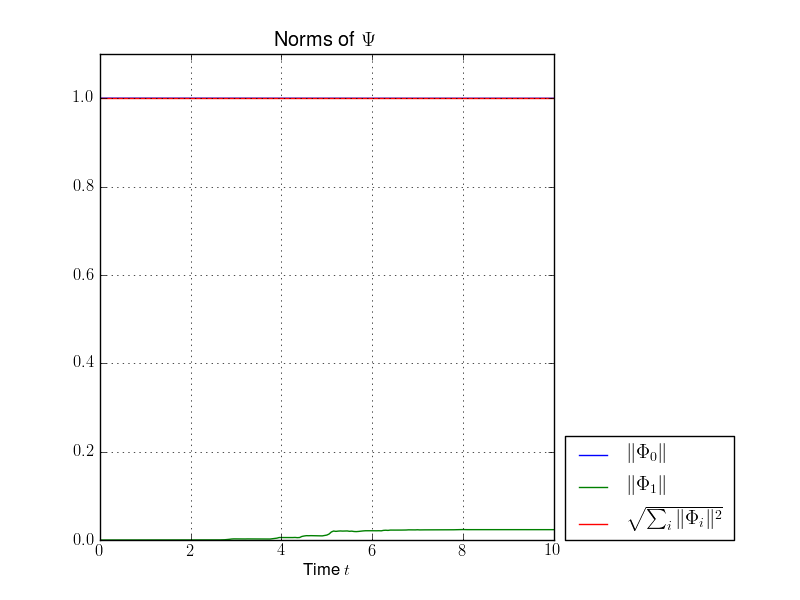
\includegraphics[width=0.5\linewidth]{./results/deltagap_rotsym/Parameters[bsize=16][eps=0-01][delta=1-0]/norms_block0.png}
  }
  \subfloat[][]{
    \label{fig:dgr_16_0-01_1-0_nd}
    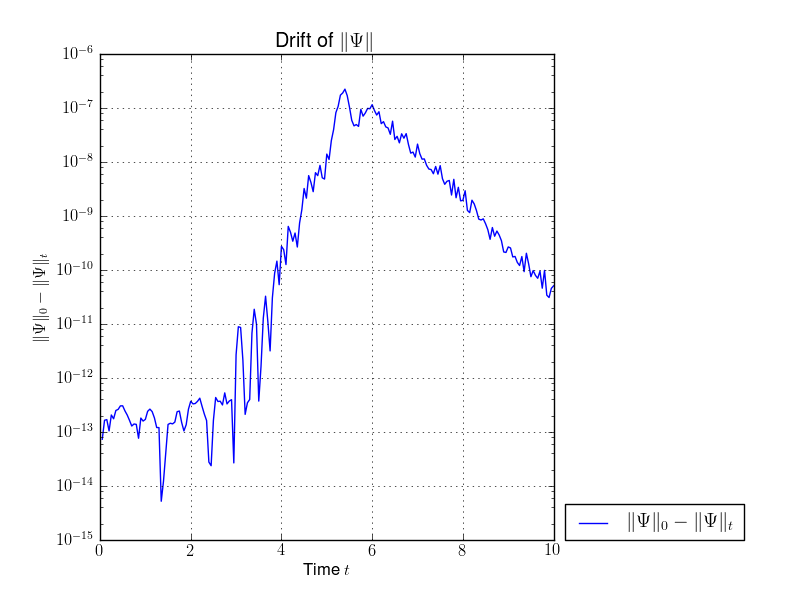
\includegraphics[width=0.5\linewidth]{./results/deltagap_rotsym/Parameters[bsize=16][eps=0-01][delta=1-0]/norms_drift_block0_log.png}
  } \\
  \caption[Plots of the norms and drifts for a simple avoided crossing]{
    Plots of the norm of the components on the upper and lower level and the drift of the total norm
    of a Gaussian wavepacket $\Ket{\Psi} = \phi_{0,0}$. The basis shape is a hyperbolic cut with cut-off $K = 16$
    and $\varepsilon = 0.01$.
    \subref{fig:dgr_16_0-01_0-2_n}, \subref{fig:dgr_16_0-01_0-2_nd} $\delta = 0.2$
    \subref{fig:dgr_16_0-01_0-5_n}, \subref{fig:dgr_16_0-01_0-5_nd} $\delta = 0.5$
    \subref{fig:dgr_16_0-01_1-0_n}, \subref{fig:dgr_16_0-01_1-0_nd} $\delta = 1.0$
%     \subref{fig:dgr_16_0-01_0-2_n} $\delta = 0.2$
%     \subref{fig:dgr_16_0-01_0-2_nd} $\delta = 0.2$
%     \subref{fig:dgr_16_0-01_0-5_n} $\delta = 0.5$
%     \subref{fig:dgr_16_0-01_0-5_nd} $\delta = 0.5$
%     \subref{fig:dgr_16_0-01_1-0_n} $\delta = 1.0$
%     \subref{fig:dgr_16_0-01_1-0_nd} $\delta = 1.0$
    \label{fig:deltagap_rotsym_16_norms_eps_001_part2}
  }
\end{figure}


\begin{figure}
  \centering
  \subfloat[][]{
    \label{fig:dgr_16_0-05_0-01_e}
    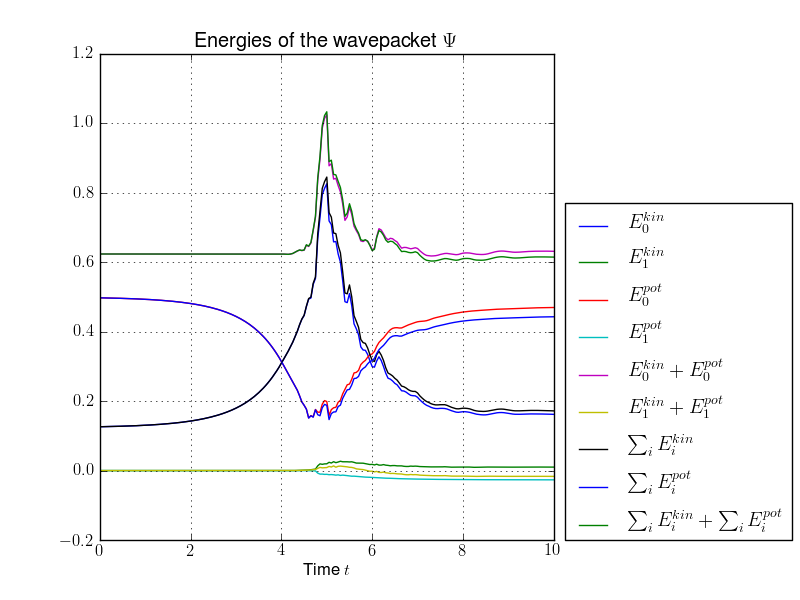
\includegraphics[width=0.5\linewidth]{./results/deltagap_rotsym/Parameters[bsize=16][eps=0-05][delta=0-01]/energies_block0.png}
  }
  \subfloat[][]{
    \label{fig:dgr_16_0-05_0-01_ed}
    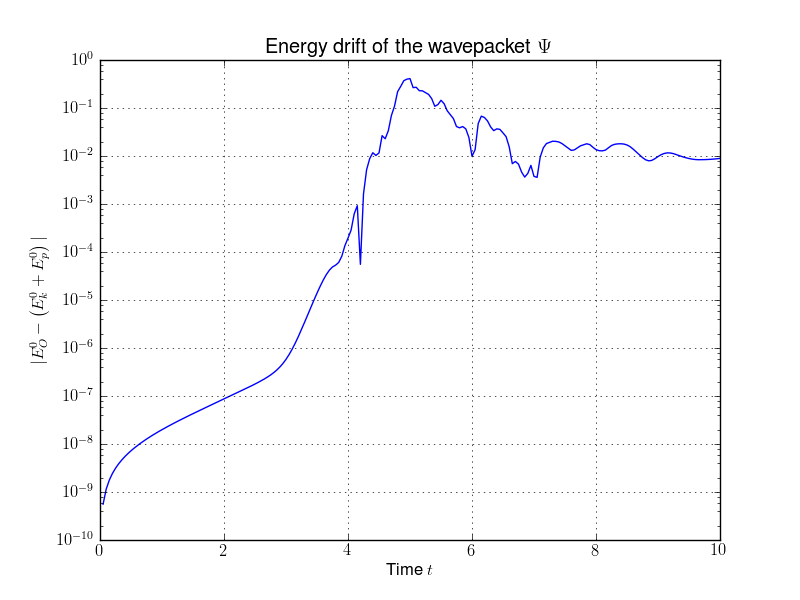
\includegraphics[width=0.5\linewidth]{./results/deltagap_rotsym/Parameters[bsize=16][eps=0-05][delta=0-01]/energy_drift_block0_log.png}
  } \\
  \subfloat[][]{
    \label{fig:dgr_16_0-05_0-05_e}
    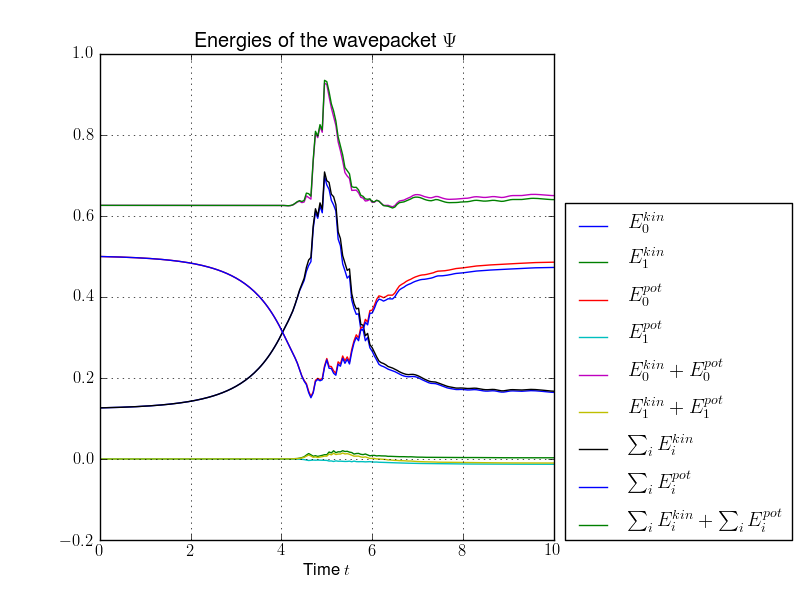
\includegraphics[width=0.5\linewidth]{./results/deltagap_rotsym/Parameters[bsize=16][eps=0-05][delta=0-05]/energies_block0.png}
  }
  \subfloat[][]{
    \label{fig:dgr_16_0-05_0-05_ed}
    \includegraphics[width=0.5\linewidth]{./results/deltagap_rotsym/Parameters[bsize=16][eps=0-05][delta=0-05]/energy_drift_block0_log.png}
  } \\
  \subfloat[][]{
    \label{fig:dgr_16_0-05_0-1_e}
    \includegraphics[width=0.5\linewidth]{./results/deltagap_rotsym/Parameters[bsize=16][eps=0-05][delta=0-1]/energies_block0.png}
  }
  \subfloat[][]{
    \label{fig:dgr_16_0-05_0-1_ed}
    \includegraphics[width=0.5\linewidth]{./results/deltagap_rotsym/Parameters[bsize=16][eps=0-05][delta=0-1]/energy_drift_block0_log.png}
  } \\
  \caption[Plots of the energies and drifts for a simple avoided crossing]{
    Plots of the kinetic, potential and total energy and the drift of the total energy
    of a Gaussian wavepacket $\Ket{\Psi} = \phi_{0,0}$. The basis shape is a hyperbolic cut with cut-off $K = 16$
    and $\varepsilon = 0.05$.
    \subref{fig:dgr_16_0-05_0-01_e}, \subref{fig:dgr_16_0-05_0-01_ed} $\delta = 0.01$
    \subref{fig:dgr_16_0-05_0-05_e}, \subref{fig:dgr_16_0-05_0-05_ed} $\delta = 0.05$
    \subref{fig:dgr_16_0-05_0-1_e}, \subref{fig:dgr_16_0-05_0-1_ed} $\delta = 0.1$
%     \subref{fig:dgr_16_0-05_0-01_e} $\delta = 0.01$
%     \subref{fig:dgr_16_0-05_0-01_ed} $\delta = 0.01$
%     \subref{fig:dgr_16_0-05_0-05_e} $\delta = 0.05$
%     \subref{fig:dgr_16_0-05_0-05_ed} $\delta = 0.05$
%     \subref{fig:dgr_16_0-05_0-1_e} $\delta = 0.1$
%     \subref{fig:dgr_16_0-05_0-1_ed} $\delta = 0.1$
    \label{fig:deltagap_rotsym_16_energies_eps_005_part1}
  }
\end{figure}


\begin{figure}
  \centering
  \subfloat[][]{
    \label{fig:dgr_16_0-05_0-2_e}
    \includegraphics[width=0.5\linewidth]{./results/deltagap_rotsym/Parameters[bsize=16][eps=0-05][delta=0-2]/energies_block0.png}
  }
  \subfloat[][]{
    \label{fig:dgr_16_0-05_0-2_ed}
    \includegraphics[width=0.5\linewidth]{./results/deltagap_rotsym/Parameters[bsize=16][eps=0-05][delta=0-2]/energy_drift_block0_log.png}
  } \\
  \subfloat[][]{
    \label{fig:dgr_16_0-05_0-5_e}
    \includegraphics[width=0.5\linewidth]{./results/deltagap_rotsym/Parameters[bsize=16][eps=0-05][delta=0-5]/energies_block0.png}
  }
  \subfloat[][]{
    \label{fig:dgr_16_0-05_0-5_ed}
    \includegraphics[width=0.5\linewidth]{./results/deltagap_rotsym/Parameters[bsize=16][eps=0-05][delta=0-5]/energy_drift_block0_log.png}
  } \\
  \subfloat[][]{
    \label{fig:dgr_16_0-05_1-0_e}
    \includegraphics[width=0.5\linewidth]{./results/deltagap_rotsym/Parameters[bsize=16][eps=0-05][delta=1-0]/energies_block0.png}
  }
  \subfloat[][]{
    \label{fig:dgr_16_0-05_1-0_ed}
    \includegraphics[width=0.5\linewidth]{./results/deltagap_rotsym/Parameters[bsize=16][eps=0-05][delta=1-0]/energy_drift_block0_log.png}
  } \\
  \caption[Plots of the energies and drifts for a simple avoided crossing]{
    Plots of the kinetic, potential and total energy and the drift of the total energy
    of a Gaussian wavepacket $\Ket{\Psi} = \phi_{0,0}$. The basis shape is a hyperbolic cut with cut-off $K = 16$
    and $\varepsilon = 0.05$.
    \subref{fig:dgr_16_0-05_0-2_e}, \subref{fig:dgr_16_0-05_0-2_ed} $\delta = 0.2$
    \subref{fig:dgr_16_0-05_0-5_e}, \subref{fig:dgr_16_0-05_0-5_ed} $\delta = 0.5$
    \subref{fig:dgr_16_0-05_1-0_e}, \subref{fig:dgr_16_0-05_1-0_ed} $\delta = 1.0$
%     \subref{fig:dgr_16_0-05_0-2_e} $\delta = 0.2$
%     \subref{fig:dgr_16_0-05_0-2_ed} $\delta = 0.2$
%     \subref{fig:dgr_16_0-05_0-5_e} $\delta = 0.5$
%     \subref{fig:dgr_16_0-05_0-5_ed} $\delta = 0.5$
%     \subref{fig:dgr_16_0-05_1-0_e} $\delta = 1.0$
%     \subref{fig:dgr_16_0-05_1-0_ed} $\delta = 1.0$
    \label{fig:deltagap_rotsym_16_energies_eps_005_part2}
  }
\end{figure}


\begin{figure}
  \centering
  \subfloat[][]{
    \label{fig:dgr_16_0-05_0-01_n}
    \includegraphics[width=0.5\linewidth]{./results/deltagap_rotsym/Parameters[bsize=16][eps=0-05][delta=0-01]/norms_block0.png}
  }
  \subfloat[][]{
    \label{fig:dgr_16_0-05_0-01_nd}
    \includegraphics[width=0.5\linewidth]{./results/deltagap_rotsym/Parameters[bsize=16][eps=0-05][delta=0-01]/norms_drift_block0_log.png}
  } \\
  \subfloat[][]{
    \label{fig:dgr_16_0-05_0-05_n}
    \includegraphics[width=0.5\linewidth]{./results/deltagap_rotsym/Parameters[bsize=16][eps=0-05][delta=0-05]/norms_block0.png}
  }
  \subfloat[][]{
    \label{fig:dgr_16_0-05_0-05_nd}
    \includegraphics[width=0.5\linewidth]{./results/deltagap_rotsym/Parameters[bsize=16][eps=0-05][delta=0-05]/norms_drift_block0_log.png}
  } \\
  \subfloat[][]{
    \label{fig:dgr_16_0-05_0-1_n}
    \includegraphics[width=0.5\linewidth]{./results/deltagap_rotsym/Parameters[bsize=16][eps=0-05][delta=0-1]/norms_block0.png}
  }
  \subfloat[][]{
    \label{fig:dgr_16_0-05_0-1_nd}
    \includegraphics[width=0.5\linewidth]{./results/deltagap_rotsym/Parameters[bsize=16][eps=0-05][delta=0-1]/norms_drift_block0_log.png}
  } \\
  \caption[Plots of the norms and drifts for a simple avoided crossing]{
    Plots of the norm of the components on the upper and lower level and the drift of the total norm
    of a Gaussian wavepacket $\Ket{\Psi} = \phi_{0,0}$. The basis shape is a hyperbolic cut with cut-off $K = 16$
    and $\varepsilon = 0.05$.
    \subref{fig:dgr_16_0-05_0-01_n}, \subref{fig:dgr_16_0-05_0-01_nd} $\delta = 0.01$
    \subref{fig:dgr_16_0-05_0-05_n}, \subref{fig:dgr_16_0-05_0-05_nd} $\delta = 0.05$
    \subref{fig:dgr_16_0-05_0-1_n}, \subref{fig:dgr_16_0-05_0-1_nd} $\delta = 0.1$
%     \subref{fig:dgr_16_0-05_0-01_n} $\delta = 0.01$
%     \subref{fig:dgr_16_0-05_0-01_nd} $\delta = 0.01$
%     \subref{fig:dgr_16_0-05_0-05_n} $\delta = 0.05$
%     \subref{fig:dgr_16_0-05_0-05_nd} $\delta = 0.05$
%     \subref{fig:dgr_16_0-05_0-1_n} $\delta = 0.1$
%     \subref{fig:dgr_16_0-05_0-1_nd} $\delta = 0.1$
    \label{fig:deltagap_rotsym_16_norms_eps_005_part1}
  }
\end{figure}


\begin{figure}
  \centering
  \subfloat[][]{
    \label{fig:dgr_16_0-05_0-2_n}
    \includegraphics[width=0.5\linewidth]{./results/deltagap_rotsym/Parameters[bsize=16][eps=0-05][delta=0-2]/norms_block0.png}
  }
  \subfloat[][]{
    \label{fig:dgr_16_0-05_0-2_nd}
    \includegraphics[width=0.5\linewidth]{./results/deltagap_rotsym/Parameters[bsize=16][eps=0-05][delta=0-2]/norms_drift_block0_log.png}
  } \\
  \subfloat[][]{
    \label{fig:dgr_16_0-05_0-5_n}
    \includegraphics[width=0.5\linewidth]{./results/deltagap_rotsym/Parameters[bsize=16][eps=0-05][delta=0-5]/norms_block0.png}
  }
  \subfloat[][]{
    \label{fig:dgr_16_0-05_0-5_nd}
    \includegraphics[width=0.5\linewidth]{./results/deltagap_rotsym/Parameters[bsize=16][eps=0-05][delta=0-5]/norms_drift_block0_log.png}
  } \\
  \subfloat[][]{
    \label{fig:dgr_16_0-05_1-0_n}
    \includegraphics[width=0.5\linewidth]{./results/deltagap_rotsym/Parameters[bsize=16][eps=0-05][delta=1-0]/norms_block0.png}
  }
  \subfloat[][]{
    \label{fig:dgr_16_0-05_1-0_nd}
    \includegraphics[width=0.5\linewidth]{./results/deltagap_rotsym/Parameters[bsize=16][eps=0-05][delta=1-0]/norms_drift_block0_log.png}
  } \\
  \caption[Plots of the norms and drifts for a simple avoided crossing]{
    Plots of the norm of the components on the upper and lower level and the drift of the total norm
    of a Gaussian wavepacket $\Ket{\Psi} = \phi_{0,0}$. The basis shape is a hyperbolic cut with cut-off $K = 16$
    and $\varepsilon = 0.05$.
    \subref{fig:dgr_16_0-05_0-2_n}, \subref{fig:dgr_16_0-05_0-2_nd} $\delta = 0.2$
    \subref{fig:dgr_16_0-05_0-5_n}, \subref{fig:dgr_16_0-05_0-5_nd} $\delta = 0.5$
    \subref{fig:dgr_16_0-05_1-0_n}, \subref{fig:dgr_16_0-05_1-0_nd} $\delta = 1.0$
%     \subref{fig:dgr_16_0-05_0-2_n} $\delta = 0.2$
%     \subref{fig:dgr_16_0-05_0-2_nd} $\delta = 0.2$
%     \subref{fig:dgr_16_0-05_0-5_n} $\delta = 0.5$
%     \subref{fig:dgr_16_0-05_0-5_nd} $\delta = 0.5$
%     \subref{fig:dgr_16_0-05_1-0_n} $\delta = 1.0$
%     \subref{fig:dgr_16_0-05_1-0_nd} $\delta = 1.0$
    \label{fig:deltagap_rotsym_16_norms_eps_005_part2}
  }
\end{figure}


\begin{figure}
  \centering
  \subfloat[][]{
    \label{fig:dgr_16_0-1_0-01_e}
    \includegraphics[width=0.5\linewidth]{./results/deltagap_rotsym/Parameters[bsize=16][eps=0-1][delta=0-01]/energies_block0.png}
  }
  \subfloat[][]{
    \label{fig:dgr_16_0-1_0-01_ed}
    \includegraphics[width=0.5\linewidth]{./results/deltagap_rotsym/Parameters[bsize=16][eps=0-1][delta=0-01]/energy_drift_block0_log.png}
  } \\
  \subfloat[][]{
    \label{fig:dgr_16_0-1_0-05_e}
    \includegraphics[width=0.5\linewidth]{./results/deltagap_rotsym/Parameters[bsize=16][eps=0-1][delta=0-05]/energies_block0.png}
  }
  \subfloat[][]{
    \label{fig:dgr_16_0-1_0-05_ed}
    \includegraphics[width=0.5\linewidth]{./results/deltagap_rotsym/Parameters[bsize=16][eps=0-1][delta=0-05]/energy_drift_block0_log.png}
  } \\
  \subfloat[][]{
    \label{fig:dgr_16_0-1_0-1_e}
    \includegraphics[width=0.5\linewidth]{./results/deltagap_rotsym/Parameters[bsize=16][eps=0-1][delta=0-1]/energies_block0.png}
  }
  \subfloat[][]{
    \label{fig:dgr_16_0-1_0-1_ed}
    \includegraphics[width=0.5\linewidth]{./results/deltagap_rotsym/Parameters[bsize=16][eps=0-1][delta=0-1]/energy_drift_block0_log.png}
  } \\
  \caption[Plots of the energies and drifts for a simple avoided crossing]{
    Plots of the kinetic, potential and total energy and the drift of the total energy
    of a Gaussian wavepacket $\Ket{\Psi} = \phi_{0,0}$. The basis shape is a hyperbolic cut with cut-off $K = 16$
    and $\varepsilon = 0.1$.
    \subref{fig:dgr_16_0-1_0-01_e}, \subref{fig:dgr_16_0-1_0-01_ed} $\delta = 0.01$
    \subref{fig:dgr_16_0-1_0-05_e}, \subref{fig:dgr_16_0-1_0-05_ed} $\delta = 0.05$
    \subref{fig:dgr_16_0-1_0-1_e}, \subref{fig:dgr_16_0-1_0-1_ed} $\delta = 0.1$
%     \subref{fig:dgr_16_0-1_0-01_e} $\delta = 0.01$
%     \subref{fig:dgr_16_0-1_0-01_ed} $\delta = 0.01$
%     \subref{fig:dgr_16_0-1_0-05_e} $\delta = 0.05$
%     \subref{fig:dgr_16_0-1_0-05_ed} $\delta = 0.05$
%     \subref{fig:dgr_16_0-1_0-1_e} $\delta = 0.1$
%     \subref{fig:dgr_16_0-1_0-1_ed} $\delta = 0.1$
    \label{fig:deltagap_rotsym_16_energies_eps_01_part1}
  }
\end{figure}


\begin{figure}
  \centering
  \subfloat[][]{
    \label{fig:dgr_16_0-1_0-2_e}
    \includegraphics[width=0.5\linewidth]{./results/deltagap_rotsym/Parameters[bsize=16][eps=0-1][delta=0-2]/energies_block0.png}
  }
  \subfloat[][]{
    \label{fig:dgr_16_0-1_0-2_ed}
    \includegraphics[width=0.5\linewidth]{./results/deltagap_rotsym/Parameters[bsize=16][eps=0-1][delta=0-2]/energy_drift_block0_log.png}
  } \\
  \subfloat[][]{
    \label{fig:dgr_16_0-1_0-5_e}
    \includegraphics[width=0.5\linewidth]{./results/deltagap_rotsym/Parameters[bsize=16][eps=0-1][delta=0-5]/energies_block0.png}
  }
  \subfloat[][]{
    \label{fig:dgr_16_0-1_0-5_ed}
    \includegraphics[width=0.5\linewidth]{./results/deltagap_rotsym/Parameters[bsize=16][eps=0-1][delta=0-5]/energy_drift_block0_log.png}
  } \\
  \subfloat[][]{
    \label{fig:dgr_16_0-1_1-0_e}
    \includegraphics[width=0.5\linewidth]{./results/deltagap_rotsym/Parameters[bsize=16][eps=0-1][delta=1-0]/energies_block0.png}
  }
  \subfloat[][]{
    \label{fig:dgr_16_0-1_1-0_ed}
    \includegraphics[width=0.5\linewidth]{./results/deltagap_rotsym/Parameters[bsize=16][eps=0-1][delta=1-0]/energy_drift_block0_log.png}
  } \\
  \caption[Plots of the energies and drifts for a simple avoided crossing]{
    Plots of the kinetic, potential and total energy and the drift of the total energy
    of a Gaussian wavepacket $\Ket{\Psi} = \phi_{0,0}$. The basis shape is a hyperbolic cut with cut-off $K = 16$
    and $\varepsilon = 0.1$.
    \subref{fig:dgr_16_0-1_0-2_e}, \subref{fig:dgr_16_0-1_0-2_ed} $\delta = 0.2$
    \subref{fig:dgr_16_0-1_0-5_e}, \subref{fig:dgr_16_0-1_0-5_ed} $\delta = 0.5$
    \subref{fig:dgr_16_0-1_1-0_e}, \subref{fig:dgr_16_0-1_1-0_ed} $\delta = 1.0$
%     \subref{fig:dgr_16_0-1_0-2_e} $\delta = 0.2$
%     \subref{fig:dgr_16_0-1_0-2_ed} $\delta = 0.2$
%     \subref{fig:dgr_16_0-1_0-5_e} $\delta = 0.5$
%     \subref{fig:dgr_16_0-1_0-5_ed} $\delta = 0.5$
%     \subref{fig:dgr_16_0-1_1-0_e} $\delta = 1.0$
%     \subref{fig:dgr_16_0-1_1-0_ed} $\delta = 1.0$
    \label{fig:deltagap_rotsym_16_energies_eps_01_part2}
  }
\end{figure}


\begin{figure}
  \centering
  \subfloat[][]{
    \label{fig:dgr_16_0-1_0-01_n}
    \includegraphics[width=0.5\linewidth]{./results/deltagap_rotsym/Parameters[bsize=16][eps=0-1][delta=0-01]/norms_block0.png}
  }
  \subfloat[][]{
    \label{fig:dgr_16_0-1_0-01_nd}
    \includegraphics[width=0.5\linewidth]{./results/deltagap_rotsym/Parameters[bsize=16][eps=0-1][delta=0-01]/norms_drift_block0_log.png}
  } \\
  \subfloat[][]{
    \label{fig:dgr_16_0-1_0-05_n}
    \includegraphics[width=0.5\linewidth]{./results/deltagap_rotsym/Parameters[bsize=16][eps=0-1][delta=0-05]/norms_block0.png}
  }
  \subfloat[][]{
    \label{fig:dgr_16_0-1_0-05_nd}
    \includegraphics[width=0.5\linewidth]{./results/deltagap_rotsym/Parameters[bsize=16][eps=0-1][delta=0-05]/norms_drift_block0_log.png}
  } \\
  \subfloat[][]{
    \label{fig:dgr_16_0-1_0-1_n}
    \includegraphics[width=0.5\linewidth]{./results/deltagap_rotsym/Parameters[bsize=16][eps=0-1][delta=0-1]/norms_block0.png}
  }
  \subfloat[][]{
    \label{fig:dgr_16_0-1_0-1_nd}
    \includegraphics[width=0.5\linewidth]{./results/deltagap_rotsym/Parameters[bsize=16][eps=0-1][delta=0-1]/norms_drift_block0_log.png}
  } \\
  \caption[Plots of the norms and drifts for a simple avoided crossing]{
    Plots of the norm of the components on the upper and lower level and the drift of the total norm
    of a Gaussian wavepacket $\Ket{\Psi} = \phi_{0,0}$. The basis shape is a hyperbolic cut with cut-off $K = 16$
    and $\varepsilon = 0.1$.
    \subref{fig:dgr_16_0-1_0-01_n}, \subref{fig:dgr_16_0-1_0-01_nd} $\delta = 0.01$
    \subref{fig:dgr_16_0-1_0-05_n}, \subref{fig:dgr_16_0-1_0-05_nd} $\delta = 0.05$
    \subref{fig:dgr_16_0-1_0-1_n}, \subref{fig:dgr_16_0-1_0-1_nd} $\delta = 0.1$
%     \subref{fig:dgr_16_0-1_0-01_n} $\delta = 0.01$
%     \subref{fig:dgr_16_0-1_0-01_nd} $\delta = 0.01$
%     \subref{fig:dgr_16_0-1_0-05_n} $\delta = 0.05$
%     \subref{fig:dgr_16_0-1_0-05_nd} $\delta = 0.05$
%     \subref{fig:dgr_16_0-1_0-1_n} $\delta = 0.1$
%     \subref{fig:dgr_16_0-1_0-1_nd} $\delta = 0.1$
    \label{fig:deltagap_rotsym_16_norms_eps_01_part1}
  }
\end{figure}


\begin{figure}
  \centering
  \subfloat[][]{
    \label{fig:dgr_16_0-1_0-2_n}
    \includegraphics[width=0.5\linewidth]{./results/deltagap_rotsym/Parameters[bsize=16][eps=0-1][delta=0-2]/norms_block0.png}
  }
  \subfloat[][]{
    \label{fig:dgr_16_0-1_0-2_nd}
    \includegraphics[width=0.5\linewidth]{./results/deltagap_rotsym/Parameters[bsize=16][eps=0-1][delta=0-2]/norms_drift_block0_log.png}
  } \\
  \subfloat[][]{
    \label{fig:dgr_16_0-1_0-5_n}
    \includegraphics[width=0.5\linewidth]{./results/deltagap_rotsym/Parameters[bsize=16][eps=0-1][delta=0-5]/norms_block0.png}
  }
  \subfloat[][]{
    \label{fig:dgr_16_0-1_0-5_nd}
    \includegraphics[width=0.5\linewidth]{./results/deltagap_rotsym/Parameters[bsize=16][eps=0-1][delta=0-5]/norms_drift_block0_log.png}
  } \\
  \subfloat[][]{
    \label{fig:dgr_16_0-1_1-0_n}
    \includegraphics[width=0.5\linewidth]{./results/deltagap_rotsym/Parameters[bsize=16][eps=0-1][delta=1-0]/norms_block0.png}
  }
  \subfloat[][]{
    \label{fig:dgr_16_0-1_1-0_nd}
    \includegraphics[width=0.5\linewidth]{./results/deltagap_rotsym/Parameters[bsize=16][eps=0-1][delta=1-0]/norms_drift_block0_log.png}
  } \\
  \caption[Plots of the norms and drifts for a simple avoided crossing]{
    Plots of the norm of the components on the upper and lower level and the drift of the total norm
    of a Gaussian wavepacket $\Ket{\Psi} = \phi_{0,0}$. The basis shape is a hyperbolic cut with cut-off $K = 16$
    and $\varepsilon = 0.1$.
    \subref{fig:dgr_16_0-1_0-2_n}, \subref{fig:dgr_16_0-1_0-2_nd} $\delta = 0.2$
    \subref{fig:dgr_16_0-1_0-5_n}, \subref{fig:dgr_16_0-1_0-5_nd} $\delta = 0.5$
    \subref{fig:dgr_16_0-1_1-0_n}, \subref{fig:dgr_16_0-1_1-0_nd} $\delta = 1.0$
%     \subref{fig:dgr_16_0-1_0-2_n} $\delta = 0.2$
%     \subref{fig:dgr_16_0-1_0-2_nd} $\delta = 0.2$
%     \subref{fig:dgr_16_0-1_0-5_n} $\delta = 0.5$
%     \subref{fig:dgr_16_0-1_0-5_nd} $\delta = 0.5$
%     \subref{fig:dgr_16_0-1_1-0_n} $\delta = 1.0$
%     \subref{fig:dgr_16_0-1_1-0_nd} $\delta = 1.0$
    \label{fig:deltagap_rotsym_16_norms_eps_01_part2}
  }
\end{figure}


\begin{figure}
  \centering
  \subfloat[][]{
    \label{fig:dgr_16_0-2_0-01_e}
    \includegraphics[width=0.5\linewidth]{./results/deltagap_rotsym/Parameters[bsize=16][eps=0-2][delta=0-01]/energies_block0.png}
  }
  \subfloat[][]{
    \label{fig:dgr_16_0-2_0-01_ed}
    \includegraphics[width=0.5\linewidth]{./results/deltagap_rotsym/Parameters[bsize=16][eps=0-2][delta=0-01]/energy_drift_block0_log.png}
  } \\
  \subfloat[][]{
    \label{fig:dgr_16_0-2_0-05_e}
    \includegraphics[width=0.5\linewidth]{./results/deltagap_rotsym/Parameters[bsize=16][eps=0-2][delta=0-05]/energies_block0.png}
  }
  \subfloat[][]{
    \label{fig:dgr_16_0-2_0-05_ed}
    \includegraphics[width=0.5\linewidth]{./results/deltagap_rotsym/Parameters[bsize=16][eps=0-2][delta=0-05]/energy_drift_block0_log.png}
  } \\
  \subfloat[][]{
    \label{fig:dgr_16_0-2_0-1_e}
    \includegraphics[width=0.5\linewidth]{./results/deltagap_rotsym/Parameters[bsize=16][eps=0-2][delta=0-1]/energies_block0.png}
  }
  \subfloat[][]{
    \label{fig:dgr_16_0-2_0-1_ed}
    \includegraphics[width=0.5\linewidth]{./results/deltagap_rotsym/Parameters[bsize=16][eps=0-2][delta=0-1]/energy_drift_block0_log.png}
  } \\
  \caption[Plots of the energies and drifts for a simple avoided crossing]{
    Plots of the kinetic, potential and total energy and the drift of the total energy
    of a Gaussian wavepacket $\Ket{\Psi} = \phi_{0,0}$. The basis shape is a hyperbolic cut with cut-off $K = 16$
    and $\varepsilon = 0.2$.
    \subref{fig:dgr_16_0-2_0-01_e}, \subref{fig:dgr_16_0-2_0-01_ed} $\delta = 0.01$
    \subref{fig:dgr_16_0-2_0-05_e}, \subref{fig:dgr_16_0-2_0-05_ed} $\delta = 0.05$
    \subref{fig:dgr_16_0-2_0-1_e}, \subref{fig:dgr_16_0-2_0-1_ed} $\delta = 0.1$
%     \subref{fig:dgr_16_0-2_0-01_e} $\delta = 0.01$
%     \subref{fig:dgr_16_0-2_0-01_ed} $\delta = 0.01$
%     \subref{fig:dgr_16_0-2_0-05_e} $\delta = 0.05$
%     \subref{fig:dgr_16_0-2_0-05_ed} $\delta = 0.05$
%     \subref{fig:dgr_16_0-2_0-1_e} $\delta = 0.1$
%     \subref{fig:dgr_16_0-2_0-1_ed} $\delta = 0.1$
    \label{fig:deltagap_rotsym_16_energies_eps_02_part1}
  }
\end{figure}


\begin{figure}
  \centering
  \subfloat[][]{
    \label{fig:dgr_16_0-2_0-2_e}
    \includegraphics[width=0.5\linewidth]{./results/deltagap_rotsym/Parameters[bsize=16][eps=0-2][delta=0-2]/energies_block0.png}
  }
  \subfloat[][]{
    \label{fig:dgr_16_0-2_0-2_ed}
    \includegraphics[width=0.5\linewidth]{./results/deltagap_rotsym/Parameters[bsize=16][eps=0-2][delta=0-2]/energy_drift_block0_log.png}
  } \\
  \subfloat[][]{
    \label{fig:dgr_16_0-2_0-5_e}
    \includegraphics[width=0.5\linewidth]{./results/deltagap_rotsym/Parameters[bsize=16][eps=0-2][delta=0-5]/energies_block0.png}
  }
  \subfloat[][]{
    \label{fig:dgr_16_0-2_0-5_ed}
    \includegraphics[width=0.5\linewidth]{./results/deltagap_rotsym/Parameters[bsize=16][eps=0-2][delta=0-5]/energy_drift_block0_log.png}
  } \\
  \subfloat[][]{
    \label{fig:dgr_16_0-2_1-0_e}
    \includegraphics[width=0.5\linewidth]{./results/deltagap_rotsym/Parameters[bsize=16][eps=0-2][delta=1-0]/energies_block0.png}
  }
  \subfloat[][]{
    \label{fig:dgr_16_0-2_1-0_ed}
    \includegraphics[width=0.5\linewidth]{./results/deltagap_rotsym/Parameters[bsize=16][eps=0-2][delta=1-0]/energy_drift_block0_log.png}
  } \\
  \caption[Plots of the energies and drifts for a simple avoided crossing]{
    Plots of the kinetic, potential and total energy and the drift of the total energy
    of a Gaussian wavepacket $\Ket{\Psi} = \phi_{0,0}$. The basis shape is a hyperbolic cut with cut-off $K = 16$
    and $\varepsilon = 0.2$.
    \subref{fig:dgr_16_0-2_0-2_e}, \subref{fig:dgr_16_0-2_0-2_ed} $\delta = 0.2$
    \subref{fig:dgr_16_0-2_0-5_e}, \subref{fig:dgr_16_0-2_0-5_ed} $\delta = 0.5$
    \subref{fig:dgr_16_0-2_1-0_e}, \subref{fig:dgr_16_0-2_1-0_ed} $\delta = 1.0$
%     \subref{fig:dgr_16_0-2_0-2_e} $\delta = 0.2$
%     \subref{fig:dgr_16_0-2_0-2_ed} $\delta = 0.2$
%     \subref{fig:dgr_16_0-2_0-5_e} $\delta = 0.5$
%     \subref{fig:dgr_16_0-2_0-5_ed} $\delta = 0.5$
%     \subref{fig:dgr_16_0-2_1-0_e} $\delta = 1.0$
%     \subref{fig:dgr_16_0-2_1-0_ed} $\delta = 1.0$
    \label{fig:deltagap_rotsym_16_energies_eps_02_part2}
  }
\end{figure}


\begin{figure}
  \centering
  \subfloat[][]{
    \label{fig:dgr_16_0-2_0-01_n}
    \includegraphics[width=0.5\linewidth]{./results/deltagap_rotsym/Parameters[bsize=16][eps=0-2][delta=0-01]/norms_block0.png}
  }
  \subfloat[][]{
    \label{fig:dgr_16_0-2_0-01_nd}
    \includegraphics[width=0.5\linewidth]{./results/deltagap_rotsym/Parameters[bsize=16][eps=0-2][delta=0-01]/norms_drift_block0_log.png}
  } \\
  \subfloat[][]{
    \label{fig:dgr_16_0-2_0-05_n}
    \includegraphics[width=0.5\linewidth]{./results/deltagap_rotsym/Parameters[bsize=16][eps=0-2][delta=0-05]/norms_block0.png}
  }
  \subfloat[][]{
    \label{fig:dgr_16_0-2_0-05_nd}
    \includegraphics[width=0.5\linewidth]{./results/deltagap_rotsym/Parameters[bsize=16][eps=0-2][delta=0-05]/norms_drift_block0_log.png}
  } \\
  \subfloat[][]{
    \label{fig:dgr_16_0-2_0-1_n}
    \includegraphics[width=0.5\linewidth]{./results/deltagap_rotsym/Parameters[bsize=16][eps=0-2][delta=0-1]/norms_block0.png}
  }
  \subfloat[][]{
    \label{fig:dgr_16_0-2_0-1_nd}
    \includegraphics[width=0.5\linewidth]{./results/deltagap_rotsym/Parameters[bsize=16][eps=0-2][delta=0-1]/norms_drift_block0_log.png}
  } \\
  \caption[Plots of the norms and drifts for a simple avoided crossing]{
    Plots of the norm of the components on the upper and lower level and the drift of the total norm
    of a Gaussian wavepacket $\Ket{\Psi} = \phi_{0,0}$. The basis shape is a hyperbolic cut with cut-off $K = 16$
    and $\varepsilon = 0.2$.
    \subref{fig:dgr_16_0-2_0-01_n}, \subref{fig:dgr_16_0-2_0-01_nd} $\delta = 0.01$
    \subref{fig:dgr_16_0-2_0-05_n}, \subref{fig:dgr_16_0-2_0-05_nd} $\delta = 0.05$
    \subref{fig:dgr_16_0-2_0-1_n}, \subref{fig:dgr_16_0-2_0-1_nd} $\delta = 0.1$
%     \subref{fig:dgr_16_0-2_0-01_n} $\delta = 0.01$
%     \subref{fig:dgr_16_0-2_0-01_nd} $\delta = 0.01$
%     \subref{fig:dgr_16_0-2_0-05_n} $\delta = 0.05$
%     \subref{fig:dgr_16_0-2_0-05_nd} $\delta = 0.05$
%     \subref{fig:dgr_16_0-2_0-1_n} $\delta = 0.1$
%     \subref{fig:dgr_16_0-2_0-1_nd} $\delta = 0.1$
    \label{fig:deltagap_rotsym_16_norms_eps_02_part1}
  }
\end{figure}


\begin{figure}
  \centering
  \subfloat[][]{
    \label{fig:dgr_16_0-2_0-2_n}
    \includegraphics[width=0.5\linewidth]{./results/deltagap_rotsym/Parameters[bsize=16][eps=0-2][delta=0-2]/norms_block0.png}
  }
  \subfloat[][]{
    \label{fig:dgr_16_0-2_0-2_nd}
    \includegraphics[width=0.5\linewidth]{./results/deltagap_rotsym/Parameters[bsize=16][eps=0-2][delta=0-2]/norms_drift_block0_log.png}
  } \\
  \subfloat[][]{
    \label{fig:dgr_16_0-2_0-5_n}
    \includegraphics[width=0.5\linewidth]{./results/deltagap_rotsym/Parameters[bsize=16][eps=0-2][delta=0-5]/norms_block0.png}
  }
  \subfloat[][]{
    \label{fig:dgr_16_0-2_0-5_nd}
    \includegraphics[width=0.5\linewidth]{./results/deltagap_rotsym/Parameters[bsize=16][eps=0-2][delta=0-5]/norms_drift_block0_log.png}
  } \\
  \subfloat[][]{
    \label{fig:dgr_16_0-2_1-0_n}
    \includegraphics[width=0.5\linewidth]{./results/deltagap_rotsym/Parameters[bsize=16][eps=0-2][delta=1-0]/norms_block0.png}
  }
  \subfloat[][]{
    \label{fig:dgr_16_0-2_1-0_nd}
    \includegraphics[width=0.5\linewidth]{./results/deltagap_rotsym/Parameters[bsize=16][eps=0-2][delta=1-0]/norms_drift_block0_log.png}
  } \\
  \caption[Plots of the norms and drifts for a simple avoided crossing]{
    Plots of the norm of the components on the upper and lower level and the drift of the total norm
    of a Gaussian wavepacket $\Ket{\Psi} = \phi_{0,0}$. The basis shape is a hyperbolic cut with cut-off $K = 16$
    and $\varepsilon = 0.2$.
    \subref{fig:dgr_16_0-2_0-2_n}, \subref{fig:dgr_16_0-2_0-2_nd} $\delta = 0.2$
    \subref{fig:dgr_16_0-2_0-5_n}, \subref{fig:dgr_16_0-2_0-5_nd} $\delta = 0.5$
    \subref{fig:dgr_16_0-2_1-0_n}, \subref{fig:dgr_16_0-2_1-0_nd} $\delta = 1.0$
%     \subref{fig:dgr_16_0-2_0-2_n} $\delta = 0.2$
%     \subref{fig:dgr_16_0-2_0-2_nd} $\delta = 0.2$
%     \subref{fig:dgr_16_0-2_0-5_n} $\delta = 0.5$
%     \subref{fig:dgr_16_0-2_0-5_nd} $\delta = 0.5$
%     \subref{fig:dgr_16_0-2_1-0_n} $\delta = 1.0$
%     \subref{fig:dgr_16_0-2_1-0_nd} $\delta = 1.0$
    \label{fig:deltagap_rotsym_16_norms_eps_02_part2}
  }
\end{figure}

We see how for larger $\varepsilon$ the energy conservation becomes worse. This is
a sign of a too small basis shape $\mathfrak{K}$ which can not capture the
emergence of more and more quantum effects. The plots of the norms show that we get
higher transition probabilities for smaller gaps $\delta$. Additionally we get faster
transitions for smaller $\varepsilon$. However we have to be careful interpreting
these results because in most simulations there is no energy conservation. Maybe
a smaller timestep $\tau$ would be appropriate in some cases.


\FloatBarrier
\section{A conical avoided crossing}

In this section we simulate a conical avoided crossing taken from
\cite{HJ_molecularpropagation} where it is classified as type 3,
see also \cite{H_classification}. The two-dimensional
potential $V(x,y)$ is given by the following real symmetric matrix:

\begin{equation} \label{eq:conic_avoided_crossing}
  \mat{V}(x,y) \assign
  \begin{pmatrix}
    x                   & \sqrt{y^2+\delta^2} \\
    \sqrt{y^2+\delta^2} & -x
  \end{pmatrix}
\end{equation}

where $\delta > 0$ is a small real number related to the gap width
which is actually $2\delta$. The effect of shrinking gap width is shown
in figure \ref{fig:conic_avoided_crossing_levels}.

\begin{figure}[ht!]
  \centering
  \includegraphics[width=0.7\linewidth]{./fig/conic_shells_0.pdf}
  \caption{Energy levels of the conic avoided crossing given by equation \eqref{eq:conic_avoided_crossing}
          for different values of $\delta$.}
  \label{fig:conic_avoided_crossing_levels}
\end{figure}

The initial parameter values are:

\begin{align*}
  \vec{q} = \begin{pmatrix}
              1 \\ 0
            \end{pmatrix}
  \quad
  \vec{p} = \begin{pmatrix}
              0 \\ 0
            \end{pmatrix}
  \quad
  \mat{Q} = \begin{pmatrix}
              1 & 0 \\ 0 & 1
            \end{pmatrix}
  \quad
  \mat{P} = \begin{pmatrix}
              i & 0 \\ 0 & i
            \end{pmatrix}
  \quad
  S = 0
\end{align*}

and we used a timestep $\tau = 0.01$.


\begin{figure}
  \centering
  \subfloat[][]{
    \label{fig:ca_32_0-01_0-01_e}
    \includegraphics[width=0.5\linewidth]{./results/conic_avoided/Parameters[bsize=32][eps=0-01][delta=0-01]/energies_block0.png}
  }
  \subfloat[][]{
    \label{fig:ca_32_0-01_0-01_ed}
    \includegraphics[width=0.5\linewidth]{./results/conic_avoided/Parameters[bsize=32][eps=0-01][delta=0-01]/energy_drift_block0_log.png}
  } \\
  \subfloat[][]{
    \label{fig:ca_32_0-01_0-05_e}
    \includegraphics[width=0.5\linewidth]{./results/conic_avoided/Parameters[bsize=32][eps=0-01][delta=0-05]/energies_block0.png}
  }
  \subfloat[][]{
    \label{fig:ca_32_0-01_0-05_ed}
    \includegraphics[width=0.5\linewidth]{./results/conic_avoided/Parameters[bsize=32][eps=0-01][delta=0-05]/energy_drift_block0_log.png}
  } \\
  \subfloat[][]{
    \label{fig:ca_32_0-01_0-1_e}
    \includegraphics[width=0.5\linewidth]{./results/conic_avoided/Parameters[bsize=32][eps=0-01][delta=0-1]/energies_block0.png}
  }
  \subfloat[][]{
    \label{fig:ca_32_0-01_0-1_ed}
    \includegraphics[width=0.5\linewidth]{./results/conic_avoided/Parameters[bsize=32][eps=0-01][delta=0-1]/energy_drift_block0_log.png}
  } \\
  \caption[Plots of the energies and drifts for a conic avoided crossing]{
    Plots of the kinetic, potential and total energy and the drift of the total energy
    of a Gaussian wavepacket $\Ket{\Psi} = \phi_{0,0}$. The basis shape is a hyperbolic cut with cut-off $K = 32$
    and $\varepsilon = 0.01$.
    \subref{fig:ca_32_0-01_0-01_e}, \subref{fig:ca_32_0-01_0-01_ed} $\delta = 0.01$
    \subref{fig:ca_32_0-01_0-05_e}, \subref{fig:ca_32_0-01_0-05_ed} $\delta = 0.05$
    \subref{fig:ca_32_0-01_0-1_e}, \subref{fig:ca_32_0-01_0-1_ed} $\delta = 0.1$
%     \subref{fig:ca_32_0-01_0-01_e} $\delta = 0.01$
%     \subref{fig:ca_32_0-01_0-01_ed} $\delta = 0.01$
%     \subref{fig:ca_32_0-01_0-05_e} $\delta = 0.05$
%     \subref{fig:ca_32_0-01_0-05_ed} $\delta = 0.05$
%     \subref{fig:ca_32_0-01_0-1_e} $\delta = 0.1$
%     \subref{fig:ca_32_0-01_0-1_ed} $\delta = 0.1$
    \label{fig:conic_avoided_32_energies_eps_001_part1}
  }
\end{figure}


\begin{figure}
  \centering
  \subfloat[][]{
    \label{fig:ca_32_0-01_0-01_n}
    \includegraphics[width=0.5\linewidth]{./results/conic_avoided/Parameters[bsize=32][eps=0-01][delta=0-01]/norms_block0.png}
  }
  \subfloat[][]{
    \label{fig:ca_32_0-01_0-01_nd}
    \includegraphics[width=0.5\linewidth]{./results/conic_avoided/Parameters[bsize=32][eps=0-01][delta=0-01]/norms_drift_block0_log.png}
  } \\
  \subfloat[][]{
    \label{fig:ca_32_0-01_0-05_n}
    \includegraphics[width=0.5\linewidth]{./results/conic_avoided/Parameters[bsize=32][eps=0-01][delta=0-05]/norms_block0.png}
  }
  \subfloat[][]{
    \label{fig:ca_32_0-01_0-05_nd}
    \includegraphics[width=0.5\linewidth]{./results/conic_avoided/Parameters[bsize=32][eps=0-01][delta=0-05]/norms_drift_block0_log.png}
  } \\
  \subfloat[][]{
    \label{fig:ca_32_0-01_0-1_n}
    \includegraphics[width=0.5\linewidth]{./results/conic_avoided/Parameters[bsize=32][eps=0-01][delta=0-1]/norms_block0.png}
  }
  \subfloat[][]{
    \label{fig:ca_32_0-01_0-1_nd}
    \includegraphics[width=0.5\linewidth]{./results/conic_avoided/Parameters[bsize=32][eps=0-01][delta=0-1]/norms_drift_block0_log.png}
  } \\
  \caption[Plots of the norms and drifts for a simple avoided crossing]{
    Plots of the norm of the components on the upper and lower level and the drift of the total norm
    of a Gaussian wavepacket $\Ket{\Psi} = \phi_{0,0}$. The basis shape is a hyperbolic cut with cut-off $K = 32$
    and $\varepsilon = 0.01$.
    \subref{fig:ca_32_0-01_0-01_n}, \subref{fig:ca_32_0-01_0-01_nd} $\delta = 0.2$
    \subref{fig:ca_32_0-01_0-05_n}, \subref{fig:ca_32_0-01_0-05_nd} $\delta = 0.5$
    \subref{fig:ca_32_0-01_0-1_n}, \subref{fig:ca_32_0-01_0-1_nd} $\delta = 1.0$
%     \subref{fig:ca_32_0-01_0-01_n} $\delta = 0.2$
%     \subref{fig:ca_32_0-01_0-01_nd} $\delta = 0.2$
%     \subref{fig:ca_32_0-01_0-05_n} $\delta = 0.5$
%     \subref{fig:ca_32_0-01_0-05_nd} $\delta = 0.5$
%     \subref{fig:ca_32_0-01_0-1_n} $\delta = 1.0$
%     \subref{fig:ca_32_0-01_0-1_nd} $\delta = 1.0$
    \label{fig:conic_avoided_32_norms_eps_001_part1}
  }
\end{figure}


\begin{figure}
  \centering
  \subfloat[][]{
    \label{fig:ca_32_0-05_0-01_e}
    \includegraphics[width=0.5\linewidth]{./results/conic_avoided/Parameters[bsize=32][eps=0-05][delta=0-01]/energies_block0.png}
  }
  \subfloat[][]{
    \label{fig:ca_32_0-05_0-01_ed}
    \includegraphics[width=0.5\linewidth]{./results/conic_avoided/Parameters[bsize=32][eps=0-05][delta=0-01]/energy_drift_block0_log.png}
  } \\
  \subfloat[][]{
    \label{fig:ca_32_0-05_0-05_e}
    \includegraphics[width=0.5\linewidth]{./results/conic_avoided/Parameters[bsize=32][eps=0-05][delta=0-05]/energies_block0.png}
  }
  \subfloat[][]{
    \label{fig:ca_32_0-05_0-05_ed}
    \includegraphics[width=0.5\linewidth]{./results/conic_avoided/Parameters[bsize=32][eps=0-05][delta=0-05]/energy_drift_block0_log.png}
  } \\
  \subfloat[][]{
    \label{fig:ca_32_0-05_0-1_e}
    \includegraphics[width=0.5\linewidth]{./results/conic_avoided/Parameters[bsize=32][eps=0-05][delta=0-1]/energies_block0.png}
  }
  \subfloat[][]{
    \label{fig:ca_32_0-05_0-1_ed}
    \includegraphics[width=0.5\linewidth]{./results/conic_avoided/Parameters[bsize=32][eps=0-05][delta=0-1]/energy_drift_block0_log.png}
  } \\
  \caption[Plots of the energies and drifts for a conic avoided crossing]{
    Plots of the kinetic, potential and total energy and the drift of the total energy
    of a Gaussian wavepacket $\Ket{\Psi} = \phi_{0,0}$. The basis shape is a hyperbolic cut with cut-off $K = 32$
    and $\varepsilon = 0.05$.
    \subref{fig:ca_32_0-05_0-01_e}, \subref{fig:ca_32_0-05_0-01_ed} $\delta = 0.01$
    \subref{fig:ca_32_0-05_0-05_e}, \subref{fig:ca_32_0-05_0-05_ed} $\delta = 0.05$
    \subref{fig:ca_32_0-05_0-1_e}, \subref{fig:ca_32_0-05_0-1_ed} $\delta = 0.1$
%     \subref{fig:ca_32_0-05_0-01_e} $\delta = 0.01$
%     \subref{fig:ca_32_0-05_0-01_ed} $\delta = 0.01$
%     \subref{fig:ca_32_0-05_0-05_e} $\delta = 0.05$
%     \subref{fig:ca_32_0-05_0-05_ed} $\delta = 0.05$
%     \subref{fig:ca_32_0-05_0-1_e} $\delta = 0.1$
%     \subref{fig:ca_32_0-05_0-1_ed} $\delta = 0.1$
    \label{fig:conic_avoided_32_energies_eps_005_part1}
  }
\end{figure}


\begin{figure}
  \centering
  \subfloat[][]{
    \label{fig:ca_32_0-05_0-01_n}
    \includegraphics[width=0.5\linewidth]{./results/conic_avoided/Parameters[bsize=32][eps=0-05][delta=0-01]/norms_block0.png}
  }
  \subfloat[][]{
    \label{fig:ca_32_0-05_0-01_nd}
    \includegraphics[width=0.5\linewidth]{./results/conic_avoided/Parameters[bsize=32][eps=0-05][delta=0-01]/norms_drift_block0_log.png}
  } \\
  \subfloat[][]{
    \label{fig:ca_32_0-05_0-05_n}
    \includegraphics[width=0.5\linewidth]{./results/conic_avoided/Parameters[bsize=32][eps=0-05][delta=0-05]/norms_block0.png}
  }
  \subfloat[][]{
    \label{fig:ca_32_0-05_0-05_nd}
    \includegraphics[width=0.5\linewidth]{./results/conic_avoided/Parameters[bsize=32][eps=0-05][delta=0-05]/norms_drift_block0_log.png}
  } \\
  \subfloat[][]{
    \label{fig:ca_32_0-05_0-1_n}
    \includegraphics[width=0.5\linewidth]{./results/conic_avoided/Parameters[bsize=32][eps=0-05][delta=0-1]/norms_block0.png}
  }
  \subfloat[][]{
    \label{fig:ca_32_0-05_0-1_nd}
    \includegraphics[width=0.5\linewidth]{./results/conic_avoided/Parameters[bsize=32][eps=0-05][delta=0-1]/norms_drift_block0_log.png}
  } \\
  \caption[Plots of the norms and drifts for a simple avoided crossing]{
    Plots of the norm of the components on the upper and lower level and the drift of the total norm
    of a Gaussian wavepacket $\Ket{\Psi} = \phi_{0,0}$. The basis shape is a hyperbolic cut with cut-off $K = 32$
    and $\varepsilon = 0.05$.
    \subref{fig:ca_32_0-05_0-01_n}, \subref{fig:ca_32_0-05_0-01_nd} $\delta = 0.2$
    \subref{fig:ca_32_0-05_0-05_n}, \subref{fig:ca_32_0-05_0-05_nd} $\delta = 0.5$
    \subref{fig:ca_32_0-05_0-1_n}, \subref{fig:ca_32_0-05_0-1_nd} $\delta = 1.0$
%     \subref{fig:ca_32_0-05_0-01_n} $\delta = 0.2$
%     \subref{fig:ca_32_0-05_0-01_nd} $\delta = 0.2$
%     \subref{fig:ca_32_0-05_0-05_n} $\delta = 0.5$
%     \subref{fig:ca_32_0-05_0-05_nd} $\delta = 0.5$
%     \subref{fig:ca_32_0-05_0-1_n} $\delta = 1.0$
%     \subref{fig:ca_32_0-05_0-1_nd} $\delta = 1.0$
    \label{fig:conic_avoided_32_norms_eps_005_part1}
  }
\end{figure}


\begin{figure}
  \centering
  \subfloat[][]{
    \label{fig:ca_32_0-1_0-01_e}
    \includegraphics[width=0.5\linewidth]{./results/conic_avoided/Parameters[bsize=32][eps=0-1][delta=0-01]/energies_block0.png}
  }
  \subfloat[][]{
    \label{fig:ca_32_0-1_0-01_ed}
    \includegraphics[width=0.5\linewidth]{./results/conic_avoided/Parameters[bsize=32][eps=0-1][delta=0-01]/energy_drift_block0_log.png}
  } \\
  \subfloat[][]{
    \label{fig:ca_32_0-1_0-05_e}
    \includegraphics[width=0.5\linewidth]{./results/conic_avoided/Parameters[bsize=32][eps=0-1][delta=0-05]/energies_block0.png}
  }
  \subfloat[][]{
    \label{fig:ca_32_0-1_0-05_ed}
    \includegraphics[width=0.5\linewidth]{./results/conic_avoided/Parameters[bsize=32][eps=0-1][delta=0-05]/energy_drift_block0_log.png}
  } \\
  \subfloat[][]{
    \label{fig:ca_32_0-1_0-1_e}
    \includegraphics[width=0.5\linewidth]{./results/conic_avoided/Parameters[bsize=32][eps=0-1][delta=0-1]/energies_block0.png}
  }
  \subfloat[][]{
    \label{fig:ca_32_0-1_0-1_ed}
    \includegraphics[width=0.5\linewidth]{./results/conic_avoided/Parameters[bsize=32][eps=0-1][delta=0-1]/energy_drift_block0_log.png}
  } \\
  \caption[Plots of the energies and drifts for a conic avoided crossing]{
    Plots of the kinetic, potential and total energy and the drift of the total energy
    of a Gaussian wavepacket $\Ket{\Psi} = \phi_{0,0}$. The basis shape is a hyperbolic cut with cut-off $K = 32$
    and $\varepsilon = 0.1$.
    \subref{fig:ca_32_0-1_0-01_e}, \subref{fig:ca_32_0-1_0-01_ed} $\delta = 0.01$
    \subref{fig:ca_32_0-1_0-05_e}, \subref{fig:ca_32_0-1_0-05_ed} $\delta = 0.05$
    \subref{fig:ca_32_0-1_0-1_e}, \subref{fig:ca_32_0-1_0-1_ed} $\delta = 0.1$
%     \subref{fig:ca_32_0-1_0-01_e} $\delta = 0.01$
%     \subref{fig:ca_32_0-1_0-01_ed} $\delta = 0.01$
%     \subref{fig:ca_32_0-1_0-05_e} $\delta = 0.05$
%     \subref{fig:ca_32_0-1_0-05_ed} $\delta = 0.05$
%     \subref{fig:ca_32_0-1_0-1_e} $\delta = 0.1$
%     \subref{fig:ca_32_0-1_0-1_ed} $\delta = 0.1$
    \label{fig:conic_avoided_32_energies_eps_01_part1}
  }
\end{figure}


\begin{figure}
  \centering
  \subfloat[][]{
    \label{fig:ca_32_0-1_0-01_n}
    \includegraphics[width=0.5\linewidth]{./results/conic_avoided/Parameters[bsize=32][eps=0-1][delta=0-01]/norms_block0.png}
  }
  \subfloat[][]{
    \label{fig:ca_32_0-1_0-01_nd}
    \includegraphics[width=0.5\linewidth]{./results/conic_avoided/Parameters[bsize=32][eps=0-1][delta=0-01]/norms_drift_block0_log.png}
  } \\
  \subfloat[][]{
    \label{fig:ca_32_0-1_0-05_n}
    \includegraphics[width=0.5\linewidth]{./results/conic_avoided/Parameters[bsize=32][eps=0-1][delta=0-05]/norms_block0.png}
  }
  \subfloat[][]{
    \label{fig:ca_32_0-1_0-05_nd}
    \includegraphics[width=0.5\linewidth]{./results/conic_avoided/Parameters[bsize=32][eps=0-1][delta=0-05]/norms_drift_block0_log.png}
  } \\
  \subfloat[][]{
    \label{fig:ca_32_0-1_0-1_n}
    \includegraphics[width=0.5\linewidth]{./results/conic_avoided/Parameters[bsize=32][eps=0-1][delta=0-1]/norms_block0.png}
  }
  \subfloat[][]{
    \label{fig:ca_32_0-1_0-1_nd}
    \includegraphics[width=0.5\linewidth]{./results/conic_avoided/Parameters[bsize=32][eps=0-1][delta=0-1]/norms_drift_block0_log.png}
  } \\
  \caption[Plots of the norms and drifts for a simple avoided crossing]{
    Plots of the norm of the components on the upper and lower level and the drift of the total norm
    of a Gaussian wavepacket $\Ket{\Psi} = \phi_{0,0}$. The basis shape is a hyperbolic cut with cut-off $K = 32$
    and $\varepsilon = 0.1$.
    \subref{fig:ca_32_0-1_0-01_n}, \subref{fig:ca_32_0-1_0-01_nd} $\delta = 0.2$
    \subref{fig:ca_32_0-1_0-05_n}, \subref{fig:ca_32_0-1_0-05_nd} $\delta = 0.5$
    \subref{fig:ca_32_0-1_0-1_n}, \subref{fig:ca_32_0-1_0-1_nd} $\delta = 1.0$
%     \subref{fig:ca_32_0-1_0-01_n} $\delta = 0.2$
%     \subref{fig:ca_32_0-1_0-01_nd} $\delta = 0.2$
%     \subref{fig:ca_32_0-1_0-05_n} $\delta = 0.5$
%     \subref{fig:ca_32_0-1_0-05_nd} $\delta = 0.5$
%     \subref{fig:ca_32_0-1_0-1_n} $\delta = 1.0$
%     \subref{fig:ca_32_0-1_0-1_nd} $\delta = 1.0$
    \label{fig:conic_avoided_32_norms_eps_01_part1}
  }
\end{figure}


\FloatBarrier
\section{A conical crossing}

In this section we show some results for a special case of the potential
\eqref{eq:conic_avoided_crossing} given in the last section. The potential
is shown in figure \ref{fig:conic_intersection}.

\begin{figure}[ht!]
  \centering
  \includegraphics[width=0.7\linewidth]{./fig/conic_intersection.pdf}
  \caption{Energy levels of the conic crossing given by equation \eqref{eq:conic_avoided_crossing}
          for $\delta = 0$. The energy levels touch for $x=y=0$.}
  \label{fig:conic_intersection}
\end{figure}

We start with a Gaussian having the following initial parameter set $\Pi$:

\begin{align*}
  \vec{q} = \begin{pmatrix}
              -0.1 \\ \alpha \varepsilon
            \end{pmatrix}
  \quad
  \vec{p} = \begin{pmatrix}
              1 \\ 0
            \end{pmatrix}
  \quad
  \mat{Q} = \begin{pmatrix}
              1 & 0 \\ 0 & 1
            \end{pmatrix}
  \quad
  \mat{P} = \begin{pmatrix}
              i & 0 \\ 0 & i
            \end{pmatrix}
  \quad
  S = 0 \,.
\end{align*}

The packet is initialised such that it misses the crossing point. This is controlled by the parameter $\alpha$ which
we will vary. Depending on this value, the potential appears to be an avoided crossing. The figures
\ref{fig:conic_missed_16_energies_smaller} and \ref{fig:conic_missed_16_energies_larger} show the energies of the
wavepacket, the figures \ref{fig:conic_missed_16_norms_smaller} and \ref{fig:conic_missed_16_norms_larger}
show the norms and transition probabilities. The time-evolution of $\Pi$ is shown in figure \ref{fig:conic_missed_pi_evolution}
while the trajectories of $\vec{q}$ are shown in figure \ref{fig:conic_missed_16_trajectories}.

\begin{figure}
  \centering
  \subfloat[][]{
    \label{fig:cm_16_0-0_0-01_e}
    \includegraphics[width=0.5\linewidth]{./results/conic_missed/Parameters[bsize=16][alpha=0-0][eps=0-01]/energies_block0.png}
  }
  \subfloat[][]{
    \label{fig:cm_16_0-0_0-01_ed}
    \includegraphics[width=0.5\linewidth]{./results/conic_missed/Parameters[bsize=16][alpha=0-0][eps=0-01]/energy_drift_block0_log.png}
  } \\
  \subfloat[][]{
    \label{fig:cm_16_0-5_0-01_e}
    \includegraphics[width=0.5\linewidth]{./results/conic_missed/Parameters[bsize=16][alpha=0-5][eps=0-01]/energies_block0.png}
  }
  \subfloat[][]{
    \label{fig:cm_16_0-5_0-01_ed}
    \includegraphics[width=0.5\linewidth]{./results/conic_missed/Parameters[bsize=16][alpha=0-5][eps=0-01]/energy_drift_block0_log.png}
  } \\
  \subfloat[][]{
    \label{fig:cm_16_1-0_0-01_e}
    \includegraphics[width=0.5\linewidth]{./results/conic_missed/Parameters[bsize=16][alpha=1-0][eps=0-01]/energies_block0.png}
  }
  \subfloat[][]{
    \label{fig:cm_16_1-0_0-01_ed}
    \includegraphics[width=0.5\linewidth]{./results/conic_missed/Parameters[bsize=16][alpha=1-0][eps=0-01]/energy_drift_block0_log.png}
  } \\
  \caption[Plots of the energies and drifts for a missed intersection]{
    Plots of the kinetic, potential and total energy and the drift of the total energy
    of a Gaussian wavepacket $\Ket{\Psi} = \phi_{0,0}$. The basis shape is a hyperbolic cut with cut-off $K = 16$
    and $\varepsilon = 0.01$.
    \subref{fig:cm_16_0-0_0-01_e}, \subref{fig:cm_16_0-0_0-01_ed} $\alpha = 0.0$
    \subref{fig:cm_16_0-5_0-01_e}, \subref{fig:cm_16_0-5_0-01_ed} $\alpha = 0.5$
    \subref{fig:cm_16_1-0_0-01_e}, \subref{fig:cm_16_1-0_0-01_ed} $\alpha = 1.0$
%     \subref{fig:cm_16_0-0_0-01_e} $\alpha = 0.0$
%     \subref{fig:cm_16_0-0_0-01_ed} $\alpha = 0.0$
%     \subref{fig:cm_16_0-5_0-01_e} $\alpha = 0.5$
%     \subref{fig:cm_16_0-5_0-01_ed} $\alpha = 0.5$
%     \subref{fig:cm_16_1-0_0-01_e} $\alpha = 1.0$
%     \subref{fig:cm_16_1-0_0-01_ed} $\alpha = 1.0$
    \label{fig:conic_missed_16_energies_smaller}
  }
\end{figure}


\begin{figure}
  \centering
  \subfloat[][]{
    \label{fig:cm_16_1-5_0-01_e}
    \includegraphics[width=0.5\linewidth]{./results/conic_missed/Parameters[bsize=16][alpha=1-5][eps=0-01]/energies_block0.png}
  }
  \subfloat[][]{
    \label{fig:cm_16_1-5_0-01_ed}
    \includegraphics[width=0.5\linewidth]{./results/conic_missed/Parameters[bsize=16][alpha=1-5][eps=0-01]/energy_drift_block0_log.png}
  } \\
  \subfloat[][]{
    \label{fig:cm_16_2-0_0-01_e}
    \includegraphics[width=0.5\linewidth]{./results/conic_missed/Parameters[bsize=16][alpha=2-0][eps=0-01]/energies_block0.png}
  }
  \subfloat[][]{
    \label{fig:cm_16_2-0_0-01_ed}
    \includegraphics[width=0.5\linewidth]{./results/conic_missed/Parameters[bsize=16][alpha=2-0][eps=0-01]/energy_drift_block0_log.png}
  } \\
  \subfloat[][]{
    \label{fig:cm_16_5-0_0-01_e}
    \includegraphics[width=0.5\linewidth]{./results/conic_missed/Parameters[bsize=16][alpha=5-0][eps=0-01]/energies_block0.png}
  }
  \subfloat[][]{
    \label{fig:cm_16_5-0_0-01_ed}
    \includegraphics[width=0.5\linewidth]{./results/conic_missed/Parameters[bsize=16][alpha=5-0][eps=0-01]/energy_drift_block0_log.png}
  } \\
  \caption[Plots of the energies and drifts for a missed intersection]{
    Plots of the kinetic, potential and total energy and the drift of the total energy
    of a Gaussian wavepacket $\Ket{\Psi} = \phi_{0,0}$. The basis shape is a hyperbolic cut with cut-off $K = 16$
    and $\varepsilon = 0.01$.
    \subref{fig:cm_16_1-5_0-01_e}, \subref{fig:cm_16_1-5_0-01_ed} $\alpha = 1.5$
    \subref{fig:cm_16_2-0_0-01_e}, \subref{fig:cm_16_2-0_0-01_ed} $\alpha = 2.0$
    \subref{fig:cm_16_5-0_0-01_e}, \subref{fig:cm_16_5-0_0-01_ed} $\alpha = 5.0$
%     \subref{fig:cm_16_1-5_0-01_e} $\alpha = 1.5$
%     \subref{fig:cm_16_1-5_0-01_ed} $\alpha = 1.5$
%     \subref{fig:cm_16_2-0_0-01_e} $\alpha = 2.0$
%     \subref{fig:cm_16_2-0_0-01_ed} $\alpha = 2.0$
%     \subref{fig:cm_16_5-0_0-01_e} $\alpha = 5.0$
%     \subref{fig:cm_16_5-0_0-01_ed} $\alpha = 5.0$
    \label{fig:conic_missed_16_energies_larger}
  }
\end{figure}


\begin{figure}
  \centering
  \subfloat[][]{
    \label{fig:cm_16_0-0_0-01_n}
    \includegraphics[width=0.5\linewidth]{./results/conic_missed/Parameters[bsize=16][alpha=0-0][eps=0-01]/norms_block0.png}
  }
  \subfloat[][]{
    \label{fig:cm_16_0-0_0-01_nd}
    \includegraphics[width=0.5\linewidth]{./results/conic_missed/Parameters[bsize=16][alpha=0-0][eps=0-01]/norms_drift_block0_log.png}
  } \\
  \subfloat[][]{
    \label{fig:cm_16_0-5_0-01_n}
    \includegraphics[width=0.5\linewidth]{./results/conic_missed/Parameters[bsize=16][alpha=0-5][eps=0-01]/norms_block0.png}
  }
  \subfloat[][]{
    \label{fig:cm_16_0-5_0-01_nd}
    \includegraphics[width=0.5\linewidth]{./results/conic_missed/Parameters[bsize=16][alpha=0-5][eps=0-01]/norms_drift_block0_log.png}
  } \\
  \subfloat[][]{
    \label{fig:cm_16_1-0_0-01_n}
    \includegraphics[width=0.5\linewidth]{./results/conic_missed/Parameters[bsize=16][alpha=1-0][eps=0-01]/norms_block0.png}
  }
  \subfloat[][]{
    \label{fig:cm_16_1-0_0-01_nd}
    \includegraphics[width=0.5\linewidth]{./results/conic_missed/Parameters[bsize=16][alpha=1-0][eps=0-01]/norms_drift_block0_log.png}
  } \\
  \caption[Plots of the norms and drifts for a missed intersection]{
    Plots of the norm of the components on the upper and lower level and the drift of the total norm
    of a Gaussian wavepacket $\Ket{\Psi} = \phi_{0,0}$. The basis shape is a hyperbolic cut with cut-off $K = 16$
    and $\varepsilon = 0.01$.
    \subref{fig:cm_16_0-0_0-01_n}, \subref{fig:cm_16_0-0_0-01_nd} $\alpha = 0.0$
    \subref{fig:cm_16_0-5_0-01_n}, \subref{fig:cm_16_0-5_0-01_nd} $\alpha = 0.5$
    \subref{fig:cm_16_1-0_0-01_n}, \subref{fig:cm_16_1-0_0-01_nd} $\alpha = 1.0$
%     \subref{fig:cm_16_0-0_0-01_n} $\alpha = 0.0$
%     \subref{fig:cm_16_0-0_0-01_nd} $\alpha = 0.0$
%     \subref{fig:cm_16_0-5_0-01_n} $\alpha = 0.5$
%     \subref{fig:cm_16_0-5_0-01_nd} $\alpha = 0.5$
%     \subref{fig:cm_16_1-0_0-01_n} $\alpha = 1.0$
%     \subref{fig:cm_16_1-0_0-01_nd} $\alpha = 1.0$
    \label{fig:conic_missed_16_norms_smaller}
  }
\end{figure}


\begin{figure}
  \centering
  \subfloat[][]{
    \label{fig:cm_16_1-5_0-01_n}
    \includegraphics[width=0.5\linewidth]{./results/conic_missed/Parameters[bsize=16][alpha=1-5][eps=0-01]/norms_block0.png}
  }
  \subfloat[][]{
    \label{fig:cm_16_1-5_0-01_nd}
    \includegraphics[width=0.5\linewidth]{./results/conic_missed/Parameters[bsize=16][alpha=1-5][eps=0-01]/norms_drift_block0_log.png}
  } \\
  \subfloat[][]{
    \label{fig:cm_16_2-0_0-01_n}
    \includegraphics[width=0.5\linewidth]{./results/conic_missed/Parameters[bsize=16][alpha=2-0][eps=0-01]/norms_block0.png}
  }
  \subfloat[][]{
    \label{fig:cm_16_2-0_0-01_nd}
    \includegraphics[width=0.5\linewidth]{./results/conic_missed/Parameters[bsize=16][alpha=2-0][eps=0-01]/norms_drift_block0_log.png}
  } \\
  \subfloat[][]{
    \label{fig:cm_16_5-0_0-01_n}
    \includegraphics[width=0.5\linewidth]{./results/conic_missed/Parameters[bsize=16][alpha=5-0][eps=0-01]/norms_block0.png}
  }
  \subfloat[][]{
    \label{fig:cm_16_5-0_0-01_nd}
    \includegraphics[width=0.5\linewidth]{./results/conic_missed/Parameters[bsize=16][alpha=5-0][eps=0-01]/norms_drift_block0_log.png}
  } \\
  \caption[Plots of the norms and drifts for a missed intersection]{
    Plots of the norm of the components on the upper and lower level and the drift of the total norm
    of a Gaussian wavepacket $\Ket{\Psi} = \phi_{0,0}$. The basis shape is a hyperbolic cut with cut-off $K = 16$
    and $\varepsilon = 0.01$.
    \subref{fig:cm_16_1-5_0-01_n}, \subref{fig:cm_16_1-5_0-01_nd} $\alpha = 1.5$
    \subref{fig:cm_16_2-0_0-01_n}, \subref{fig:cm_16_2-0_0-01_nd} $\alpha = 2.0$
    \subref{fig:cm_16_5-0_0-01_n}, \subref{fig:cm_16_5-0_0-01_nd} $\alpha = 5.0$
%     \subref{fig:cm_16_1-5_0-01_n} $\alpha = 1.5$
%     \subref{fig:cm_16_1-5_0-01_nd} $\alpha = 1.5$
%     \subref{fig:cm_16_2-0_0-01_n} $\alpha = 2.0$
%     \subref{fig:cm_16_2-0_0-01_nd} $\alpha = 2.0$
%     \subref{fig:cm_16_5-0_0-01_n} $\alpha = 5.0$
%     \subref{fig:cm_16_5-0_0-01_nd} $\alpha = 5.0$
    \label{fig:conic_missed_16_norms_larger}
  }
\end{figure}


\begin{figure}
  \centering
  \includegraphics[width=\linewidth]{./results/conic_missed/Parameters[bsize=16][alpha=1-0][eps=0-01]/wavepacket_parameters_abs_ang_block0.png}
  \caption[Time-evolution of the parameter set $\Pi$]{
    Time-evolution of the parameter set $\Pi$. The curves look similar for all values of $\alpha$.}
  \label{fig:conic_missed_pi_evolution}
\end{figure}


\begin{figure}
  \centering
  \subfloat[][]{
    \label{fig:cm_16_0-0_0-01_tq}
    \includegraphics[width=0.5\linewidth]{./results/conic_missed/Parameters[bsize=16][alpha=0-0][eps=0-01]/wavepacket_parameters_trajectoryq_block0.png}
  }
  \subfloat[][]{
    \label{fig:cm_16_0-5_0-01_tq}
    \includegraphics[width=0.5\linewidth]{./results/conic_missed/Parameters[bsize=16][alpha=0-5][eps=0-01]/wavepacket_parameters_trajectoryq_block0.png}
  } \\
  \subfloat[][]{
    \label{fig:cm_16_1-0_0-01_tq}
    \includegraphics[width=0.5\linewidth]{./results/conic_missed/Parameters[bsize=16][alpha=1-0][eps=0-01]/wavepacket_parameters_trajectoryq_block0.png}
  }
  \subfloat[][]{
    \label{fig:cm_16_1-5_0-01_tq}
    \includegraphics[width=0.5\linewidth]{./results/conic_missed/Parameters[bsize=16][alpha=1-5][eps=0-01]/wavepacket_parameters_trajectoryq_block0.png}
  } \\
  \subfloat[][]{
    \label{fig:cm_16_2-0_0-01_tq}
    \includegraphics[width=0.5\linewidth]{./results/conic_missed/Parameters[bsize=16][alpha=2-0][eps=0-01]/wavepacket_parameters_trajectoryq_block0.png}
  }
  \subfloat[][]{
    \label{fig:cm_16_5-0_0-01_tq}
    \includegraphics[width=0.5\linewidth]{./results/conic_missed/Parameters[bsize=16][alpha=5-0][eps=0-01]/wavepacket_parameters_trajectoryq_block0.png}
  } \\
  \caption[Trajectories of position for a missed intersection]{
    The trajectories of $\vec{q}$ of a Gaussian wavepacket $\Ket{\Psi} = \phi_{0,0}$ in the $x$-$y$-plane.
    The basis shape is a hyperbolic cut with cut-off $K = 16$ and $\varepsilon = 0.01$.
    \subref{fig:cm_16_0-0_0-01_tq} $\alpha = 0.0$
    \subref{fig:cm_16_0-5_0-01_tq} $\alpha = 0.5$
    \subref{fig:cm_16_1-0_0-01_tq} $\alpha = 1.0$
    \subref{fig:cm_16_1-5_0-01_tq} $\alpha = 1.5$
    \subref{fig:cm_16_2-0_0-01_tq} $\alpha = 2.0$
    \subref{fig:cm_16_5-0_0-01_tq} $\alpha = 5.0$
    \label{fig:conic_missed_16_trajectories}
  }
\end{figure}


\FloatBarrier
\subsection{A special initial condition}


In this small section we show a simulation result for a very
specialised, unnatural initial configuration. The parameter set $\Pi$ is:

\begin{align*}
  \vec{q} = \begin{pmatrix}
              -\alpha \varepsilon \\ \alpha \varepsilon
            \end{pmatrix}
  \quad
  \vec{p} = \begin{pmatrix}
              0.1 \\ 0.1
            \end{pmatrix}
  \quad
  \mat{Q} = \begin{pmatrix}
              1 & 0 \\ 0 & 1
            \end{pmatrix}
  \quad
  \mat{P} = \begin{pmatrix}
              i & 0 \\ 0 & i
            \end{pmatrix}
  \quad
  S = 0
\end{align*}

with $\alpha = 2.0$ and $\varepsilon=0.01$. We take a Gaussian wavepacket $\Ket{\Psi} = \phi_{0,0}$
for this experiment.

\begin{figure}[ht!]
  \centering
  \subfloat[][]{
    \label{fig:circle_tq}
    \includegraphics[width=0.5\linewidth]{./results/conic_circle/wavepacket_parameters_trajectoryq_block0.png}
  }
  \subfloat[][]{
    \label{fig:circle_tp}
    \includegraphics[width=0.5\linewidth]{./results/conic_circle/wavepacket_parameters_trajectoryp_block0.png}
  } \\
  \caption[Trajectories of position and momentum for a special setting]{
    The trajectories of $\vec{q}$ and $\vec{p}$ in the $x$-$y$-plane.
    \label{fig:conic_circle_trajectories}
  }
\end{figure}

\begin{figure}[ht!]
  \centering
  \subfloat[][]{
    \label{fig:circle_tQ}
    \includegraphics[width=0.5\linewidth]{./results/conic_circle/wavepacket_parameters_trajectoryQ_block0.png}
  }
  \subfloat[][]{
    \label{fig:circle_tP}
    \includegraphics[width=0.5\linewidth]{./results/conic_circle/wavepacket_parameters_trajectoryP_block0.png}
  } \\
  \caption[Trajectories of the spreads for a special setting]{
    The trajectories of $\det\mat{Q}$ and $\det\mat{P}$ in the complex plane.
    \label{fig:conic_circle_trajectories_spreads}
  }
\end{figure}

\begin{figure}
  \centering
  \includegraphics[width=\linewidth]{./results/conic_circle/wavepacket_parameters_abs_ang_block0.png}
  \caption{Time-evolution of the parameter set $\Pi$ for a special setting}
  \label{fig:conic_circle_parameters}
\end{figure}

\begin{figure}
  \centering
  \subfloat[][]{
    \label{fig:circle_e}
    \includegraphics[width=0.5\linewidth]{./results/conic_circle/energies_block0.png}
  }
  \subfloat[][]{
    \label{fig:circle_n}
    \includegraphics[width=0.5\linewidth]{./results/conic_circle/norms_block0.png}
  } \\
  \caption[Energies and norms for a special setting]{
    The plots show the energies and norms of a very special initial setting
    where the packet orbits around the crossing point.
    \label{fig:conic_circle}
  }
\end{figure}


\FloatBarrier
\section{Higher dimensional conical avoided crossings}

We can generalise the potential given in \eqref{eq:conic_avoided_crossing}
to an arbitrary number $D$ of dimensions. The matrix looks like:

\begin{equation} \label{eq:conic_avoided_crossing_DD}
  \mat{V}(\vec{x}) \assign
  \begin{pmatrix}
    x_0                                      & \sqrt{\delta^2 + \sum_{d=1}^{D-1} x_d^2} \\
    \sqrt{\delta^2 + \sum_{d=1}^{D-1} x_d^2} & -x_0
  \end{pmatrix} \,.
\end{equation}

In the following we show a three-dimensional example. The parameters are initialised to:

\begin{align*}
  \vec{q} = \begin{pmatrix}
              1.0 \\ 0 \\ 0
            \end{pmatrix}
  \quad
  \vec{p} = \begin{pmatrix}
              0 \\ 0 \\ 0
            \end{pmatrix}
  \quad
  \mat{Q} = \begin{pmatrix}
              1.0 & 0 & 0 \\ 0 & 1.0 & 0 \\ 0 & 0 & 1.0
            \end{pmatrix}
  \quad
  \mat{P} = \begin{pmatrix}
              i & 0 & 0 \\ 0 & i & 0 \\ 0 & 0 & i
            \end{pmatrix}
  \quad
  S = 0
\end{align*}

and $\varepsilon = 0.01$. The timestep is set to $\tau = 0.01$ and we use a hyperbolic cut
basis shape with cut-off $K = 16$. The energy gap is taken to be $\delta = 0.5$.

\begin{figure}
  \centering
  \subfloat[][]{
    \label{fig:ca3d_energies}
    \includegraphics[width=0.5\linewidth]{./results/conic_avoided_3d/energies_block0.png}
  }
  \subfloat[][]{
    \label{fig:ca3d_energy_drift}
    \includegraphics[width=0.5\linewidth]{./results/conic_avoided_3d/energy_drift_block0_log.png}
  } \\
  \caption[Energies of a wavepacket in athree-dimensional conical avoided crossing]
          {The kinetic, potential and total energy and the drift of the
           total energy of a wavepacket in a three-dimensional conical avoided crossing.
    \subref{fig:ca3d_energies} The energies.
    \subref{fig:ca3d_energy_drift} The energy drift.
    \label{fig:ca3d_energy_plots}
  }
\end{figure}


\begin{figure}
  \centering
  \subfloat[][]{
    \label{fig:ca3d_norms}
    \includegraphics[width=0.5\linewidth]{./results/conic_avoided_3d/norms_block0.png}
  }
  \subfloat[][]{
    \label{fig:ca3d_norms_drift}
    \includegraphics[width=0.5\linewidth]{./results/conic_avoided_3d/norms_drift_block0_log.png}
  } \\
  \caption[Norms of a wavepacket in a three-dimensional conical avoided crossing]{
    Plots of the norm of the components on the upper and lower level and the drift of the total norm
    of a Gaussian wavepacket $\Ket{\Psi} = \phi_{0,0}$ in a three-dimensional conical avoided crossing.
    \subref{fig:ca3d_norms} The norms.
    \subref{fig:ca3d_norms_drift} The norm drift.
    \label{fig:ca3d_norms_plots}
  }
\end{figure}

\begin{figure}
  \centering
  \includegraphics[width=\linewidth]{./results/conic_avoided_3d/wavepacket_parameters_abs_ang_block0.png}
  \caption{Time-evolution of the parameter set $\Pi$ of a wavepacket in a
           three-dimensional conical avoided crossing.}
  \label{fig:ca3d_parameters}
\end{figure}

\begin{figure}
  \centering
  \subfloat[][]{
    \label{fig:ca3d_traject_Q}
    \includegraphics[width=0.5\linewidth]{./results/conic_avoided_3d/wavepacket_parameters_trajectoryQ_block0.png}
  }
  \subfloat[][]{
    \label{fig:ca3d_traject_P}
    \includegraphics[width=0.5\linewidth]{./results/conic_avoided_3d/wavepacket_parameters_trajectoryP_block0.png}
  } \\
  \caption[Trajectories of the spread matrices]{
    Trajectories of $\det\mat{Q}$ and $\det\mat{P}$ in the complex plane.
    \subref{fig:ca3d_traject_Q} Trajectory of $\det\mat{Q}$.
    \subref{fig:ca3d_traject_P} Trajectory of $\det\mat{P}$.
    \label{fig:ca3d_traject_QP}
  }
\end{figure}


\FloatBarrier
\section{Examples from chemistry}


We are currently working on some real world examples directly taken from chemistry.
Most recent work is done on the example of Pyrazine, studied extensively in
\cite{Lasser, lee_heller, westermann, Xie_Guo_Amatatsu_Kosloff}. Some other interesting
problems are presented in \cite{Sardar, Adhikari}. The results of these efforts will be
published elsewhere.
